%% 
%% Copyright 2007-2020 Elsevier Ltd
%% 
%% This file is part of the 'Elsarticle Bundle'.
%% ---------------------------------------------
%% 
%% It may be distributed under the conditions of the LaTeX Project Public
%% License, either version 1.2 of this license or (at your option) any
%% later version.  The latest version of this license is in
%%    http://www.latex-project.org/lppl.txt
%% and version 1.2 or later is part of all distributions of LaTeX
%% version 1999/12/01 or later.
%% 
%% The list of all files belonging to the 'Elsarticle Bundle' is
%% given in the file `manifest.txt'.
%% 

%% Template article for Elsevier's document class `elsarticle'
%% with numbered style bibliographic references
%% SP 2008/03/01
%%
%% 
%%
%% $Id: elsarticle-template-num.tex 190 2020-11-23 11:12:32Z rishi $
%%
%%
\documentclass[preprint,12pt]{elsarticle}

%% Use the option review to obtain double line spacing
%% \documentclass[authoryear,preprint,review,12pt]{elsarticle}

%% Use the options 1p,twocolumn; 3p; 3p,twocolumn; 5p; or 5p,twocolumn
%% for a journal layout:
%% \documentclass[final,1p,times]{elsarticle}
%% \documentclass[final,1p,times,twocolumn]{elsarticle}
%% \documentclass[final,3p,times]{elsarticle}
%% \documentclass[final,3p,times,twocolumn]{elsarticle}
%% \documentclass[final,5p,times]{elsarticle}
%% \documentclass[final,5p,times,twocolumn]{elsarticle}

%% For including figures, graphicx.sty has been loaded in
%% elsarticle.cls. If you prefer to use the old commands
%% please give \usepackage{epsfig}

%% The amssymb package provides various useful mathematical symbols
\usepackage{amssymb,graphicx,amsmath,gensymb}
\usepackage[table]{xcolor}
\usepackage{booktabs}
\usepackage[margin=0.75in]{geometry}
\usepackage{todonotes,tabularx}


%% The amsthm package provides extended theorem environments
%% \usepackage{amsthm}

%% The lineno packages adds line numbers. Start line numbering with
%% \begin{linenumbers}, end it with \end{linenumbers}. Or switch it on
%% for the whole article with \linenumbers.
%% \usepackage{lineno}

\journal{Sustainable Cities and Society}

\begin{document}

\begin{frontmatter}

%% Title, authors and addresses

%% use the tnoteref command within \title for footnotes;
%% use the tnotetext command for theassociated footnote;
%% use the fnref command within \author or \address for footnotes;
%% use the fntext command for theassociated footnote;
%% use the corref command within \author for corresponding author footnotes;
%% use the cortext command for theassociated footnote;
%% use the ead command for the email address,
%% and the form \ead[url] for the home page:
%% \title{Title\tnoteref{label1}}
%% \tnotetext[label1]{}
%% \author{Name\corref{cor1}\fnref{label2}}
%% \ead{email address}
%% \ead[url]{home page}
%% \fntext[label2]{}
%% \cortext[cor1]{}
%% \affiliation{organization={},
%%             addressline={},
%%             city={},
%%             postcode={},
%%             state={},
%%             country={}}
%% \fntext[label3]{}

\title{Automated Urban Energy Assessment: From Thermal Flyover to AI-Driven Retrofit
  Prioritization for Sustainable Cities}

%% use optional labels to link authors explicitly to addresses:
%% \author[label1,label2]{}
%% \affiliation[label1]{organization={},
%%             addressline={},
%%             city={},
%%             postcode={},
%%             state={},
%%             country={}}
%%
%% \affiliation[label2]{organization={},
%%             addressline={},
%%             city={},
%%             postcode={},
%%             state={},
%%             country={}}

% \affiliation[inst1]{organization={Department of Architecture, Faculty of Architecture, The University of Hong Kong},%Department and Organization
%             addressline={Knowles Building}, 
%             city={Hong Kong SAR},
%             % postcode={00000}, 
%             % state={State One},
%             country={China}}

% \author[inst1]{Hongshan Guo}
% \author[inst2]{Sebastiano Anselmo}
% \author[inst3]{Maria Ferrara}
% \author[inst1]{Shuai Niu}
% \author[inst1]{Binlin Chi}
% \author[inst1]{Xuchen Wang}

% \affiliation[inst2]{organization={Interuniversity Department of Regional and Urban Studies and Planning, Politecnico di Turin},%Department and Organization
%             addressline={Viale Mattioli 39}, 
%             city={Turin},
%             % postcode={22222}, 
%             % state={State Two},
%             country={Italy}}

% \affiliation[inst3]{organization={Department of Energy, Politecnico di Turin},%Department and Organization
%             addressline={Corso Duca degli Abruzzi 24}, 
%             city={Turin},
%             % postcode={22222}, 
%             % state={State Two},
%             country={Italy}}
\begin{graphicalabstract}
    \includegraphics[width=\textwidth]{img/Segment.png}
    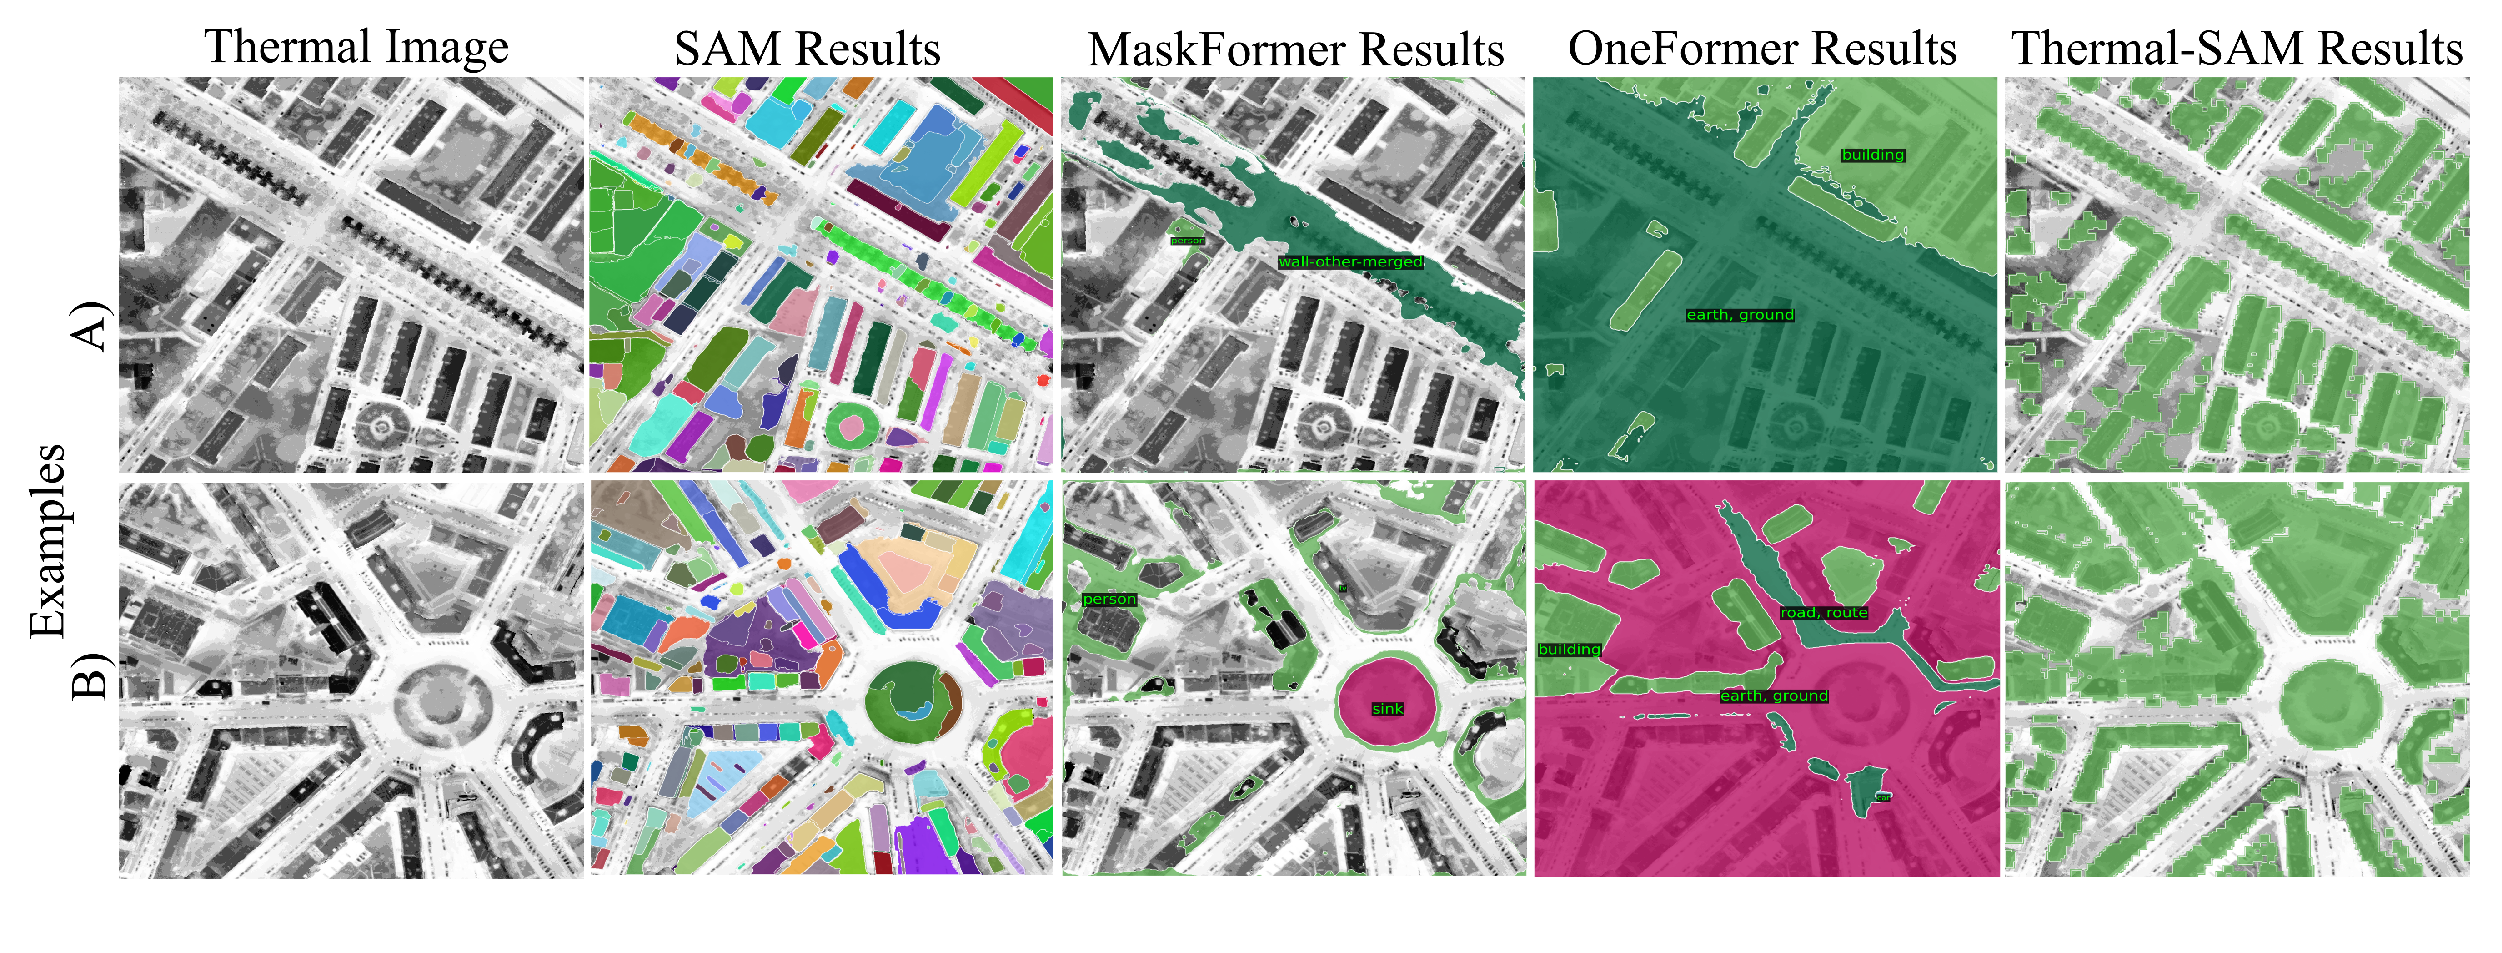
\includegraphics[width=\textwidth]{img/eval_baseline.pdf}
    \includegraphics[width=0.5\textwidth]{img/comparison_overlay_1010.png}
    \includegraphics[width=0.5\textwidth]{img/comparison_overlay_1002.png}
\end{graphicalabstract}

\begin{highlights}
\item Unsupervised pipeline fuses aerial RGB and mid-IR to extract façade thermal patches (no labels)
\item Thermal-ring features (ring mean, gradient, percentile) capture heat-loss patterns
\item CatBoost on thermal-ring features: RMSE34.4 kWh/m²·yr, MAPE19\%, EPC class accuracy62\% ($\pm$1 band90\%)
\item Three ring features (mean temp, gradient, 95th percentile) contribute 72\% of model gain
\item Open-source code for EPC cleaning and segmentation enables block-level EUI estimation from a flyover
\end{highlights}

\begin{abstract}
\noindent
  Cities urgently need scalable methods to assess building energy performance for retrofit
  prioritization, yet current approaches are costly and slow for comprehensive urban planning.
  We present an automated pipeline that transforms thermal flyovers into actionable energy
  assessments using AI-driven analysis.

  Our approach segments mid-wave infrared orthomosaics into building patches, extracts
  physically interpretable "thermal-ring" features, and predicts energy-use intensity (EUI)
  with gradient boosting. Validated on 1,168 residential buildings in Turin's post-war social
  housing district, our CatBoost model achieves 34.4~kWhm$^{-2}$yr$^{-1}$ RMSE and 19\% MAPE using only
  thermal features—matching EPC-based benchmarks without on-site data collection. Energy class
  accuracy reaches 62\% (90\% within ±1 band).

  Three thermal-ring metrics explain 72\% of predictive power, demonstrating clear physical
  interpretability. By enabling rapid district-wide screening from single aircraft campaigns,
  this framework supports municipal retrofit prioritization and policy monitoring at
  unprecedented scale. Open-source code facilitates EU-wide deployment for sustainable urban
  energy planning.


\end{abstract}


\begin{keyword}
%% keywords here, in the form: keyword \sep keyword
sustainable cities \sep urban energy planning \sep thermal imagery \sep Energy Usage Intensity \sep retrofit prioritization \sep computer vision
\end{keyword}

\end{frontmatter}
%__ Introduction
\begin{table}[htbp]
  \centering
  \caption{Nomenclature}
  \begin{tabularx}{\textwidth}{@{}lX@{}}
    \toprule
    \textbf{Abbreviation} & \textbf{Definition} \\ \midrule
    AutoML & Automated Machine Learning \\[0.4em]
    BLIP2 & Bootstrapping Language-Image Pre-training with Frozen Image Encoders and Large Language Models \\[0.4em]
    CatBoost & Categorical Gradient Boosting algorithm \\[0.4em]
    CLIP-Segment & Contrastive Language-Image Pre-training for Image Segmentation \\[0.4em]
    CNN   & Convolutional Neural Network \\[0.4em]
    ENEA  & Italian National Agency for New Technologies, Energy, and Sustainable Development \\[0.4em]
    EPC   & Energy Performance Certificate \\[0.4em]
    EUI   & Energy Usage Intensity (kWh\,m$^{-2}$\,yr$^{-1}$) \\[0.4em]
    IFOV  & Instantaneous Field of View \\[0.4em]
    MAPE  & Mean Absolute Percentage Error \\[0.4em]
    MWIR  & Mid-Wave Infrared (3–5 µm) \\[0.4em]
    OneFormer & Transformer-based model for universal image segmentation \\[0.4em]
    RGB   & Red, Green, Blue color channels \\[0.4em]
    RMSE  & Root-Mean-Square Error \\[0.4em]
    RNN   & Recurrent Neural Network \\[0.4em]
    SAM   & Segment Anything Model \\[0.4em]
    Sentence Transformer & Model for generating semantically meaningful sentence embeddings \\[0.4em]
    SIAPE & \textit{Sistema Informativo sugli Attestati di Prestazione Energetica} \\[0.4em]
    WGS84 & World Geodetic System 1984 \\[0.4em]
    \bottomrule
  \end{tabularx}
  \label{tab:nomenclature}
\end{table}


\section{Introduction}%CLC
    Buildings account for 40\% of final energy consumption and 36\% of energy-related greenhouse 
  gas emissions worldwide, making them crucial for carbon reduction—particularly within the 
  EU's commitment to climate neutrality by 2050. Municipal decision-makers face mounting 
  pressure to retrofit aging building stock under the EU Green Deal framework, which targets 35
   million buildings for renovation by 2030. The Energy Performance Certificate (EPC), mandated
   by the Energy Performance of Buildings Directive (EPBD), serves as the primary regulatory 
  tool for energy assessment. However, traditional building-by-building energy audits cannot 
  scale to comprehensive urban planning requirements. While EPCs enable energy-saving 
  opportunities and promote low-carbon building practices, challenges persist: incomplete 
  coverage, data quality issues from self-reported values, and significant gaps for uncertified
   buildings limit their utility for systematic municipal energy planning and retrofit 
  prioritization.

        
    In the meantime, the interest in predicting Energy Usage Intensity (EUIs from here on) continues to rise. Within the multitude of options more and more researchers have become more and more interested in leveraging the EPCs due to the level of detail that it provides \cite{sylten_wikell_predicting_2024} but often seen to be heavily reliant on data cleaning and pre-processing due to the inherent complexity of EPC data. This is particularly true as many of those information are self-reported and may even end up using default values that are not representative, thus creating a significant hurdle for modelers to overcome in data cleaning before any models can be trained and evaluated. Finding the right set of information that would allow for building-scale feature extraction and engineering for EPC records that are building/unit specific therefore becomes a problem that is worth investigating. In our study, EPC data are used exclusively for two purposes: (1) to compute the target variable (EUI) and (2) to geospatially locate each building unit. No additional EPC attributes are incorporated into the feature engineering process.
        
    Recognizing thermal imagery as an obvious parallel source of information that theoretically can enhance what EPC data can provide when predicting energy usage, we hope to assess its validity in providing an alternative source of information that compliment the existing EPC records. This is however not a step that further enhances the EPC record as was seen in cases like SmartEPC\cite{energinvest2024smartEPC}, but rather a parallel process that identifies alternative sources of features that helps predict energy usage intensity of buildings/units. However, despite thermal imagery's common usage in envelope diagnostics \cite{jeong_development_2017}, there is very little existing research on how to leverage thermal imagery for block-specific energy usage prediction. In particular, methods for segmenting thermal imagery collected from aircrafts are essentially nonexistent, as most remote-sensing studies relying on satellite-based high-resolution visual data and cannot be applied to thermal imagery which often have far worse resolution due to spectrum constraints. We would like to address this critical knowledge gap, and attempt to accurately segment thermal imagery at the building level to feed into EUI prediction models. 

    Our novel framework leverages thermal imagery-derived features to predict building-level Energy Usage Intensity (EUI). It is important to clarify that our approach is not designed to directly compare predictions derived solely from EPC data. Instead, EPC records—despite their inherent limitations and the need for substantial data aggregation—are used exclusively to compute a benchmark target EUI for each building via geospatial matching and averaging of multiple EPC entries. This indirect approach acknowledges the poor data quality and aggregation issues of EPCs, making a direct EPC-only prediction both infeasible and non-representative. By demonstrating that our thermal image-based predictions achieve satisfactory error metrics against these benchmark targets, we highlight the potential of our method as a scalable alternative for urban energy assessment.
    
    As we address this segmentation challenge, our study aims to enhance building energy performance predictions by integrating thermal imagery to EPC data. We will be focusing also on a novel application of unsupervised multi-modal segmentation techniques. Using Turin, Italy as a case study, we will attempt to answer the following questions: 1. How can thermal imagery segmentation using unsupervised multi-modal models improve large-scale urban energy assessments? 2. How can the segmented thermal imagery be effectively integrated with existing EPC data to improve the accuracy of Energy Use Intensity (EUI) predictions in urban buildings? 3. What are the implications of this novel approach for urban energy policy and planning? In addressing these questions, we seek to develop a more accurate and scalable approach that allows for accurate EUI prediction, which we believe is not only valuable to researchers, but also helpful for setting up energy efficiency strategies and policy-making in cities worldwide.  

%__ Background
\section{Background}
% __Refreshed Lit
    \subsection{Energy Performance Certificate and its Predictive Power}%CLC
    The Energy Performance Certificate, also known as Attestato di Prestazione Energetica in Italy, has been a cornerstone of energy certification legislation in Europe since its introduction by the EU's Energy Performance of Buildings Directive (EPBD), which sets out a framework for assessing the energy performance of buildings\cite{lavecchia_predicting_2024}, reflecting the EU's commitment to reducing energy consumption and promoting energy efficiency in buildings. In Italy, it is required for all buildings, residential and non-residential, to file for EPC whenever they are sold, rented or put under major renovation \cite{lavecchia_predicting_2024}. The filing process demands a record on the unit's energy performance on items such as energy class, actual consumption and recommendations for improving energy efficiency. Upon filing, the EPC is then valid for ten years but will need refiling when there're significant changes made to the building's energy systems or envelope.

    There are several known challenges and limitations with the collection of EPCs in Italy nonetheless. First up is the reliability of the records filed that ended up generating the certificates\cite{few_over-prediction_2023}. In some cases, EPCs values are flawed by data unavailability on the energy system or default values for the u-values, while in other cases some fields are not filled in, thus resulting in null values. This clearly also means the quality of the EPCs, in particular what fields can be relied upon for energy prediction cannot be determined, even when assuming fields related to EUI calculations are all reliable and error-free. This can lead to obvious discrepancies between the estimated and actual energy consumption from EPCs, which further limit the usefulness of EPC as a useful datasource of predicting EUIs. 

    In the meantime, it is also important to note that the coverage of EPC records is inherently not very reliable. 
    Furthermore, the coverage of EPC records is incomplete. While regulatory requirements mandate certification under specific circumstances (e.g., when buildings are sold, rented, or undergo major renovation ), not all buildings in Italy possess an EPC, particularly older buildings or those in rural areas that have not undergone such events.
    The format and availability of EPC data can also vary across regions, making it difficult to collate various reports into one comprehensive dataset for EUI prediction/energy usage classification. At such, despite certain successful case studies and attempts in leveraging EPC data to predict building energy usage\cite{araujo_optimizing_2024,gonzalez_caceres_usability_2018}, the methodology itself did not gain much popularity amongst researchers.

    Nonetheless, to establish a benchmark for EPC-based EUI prediction performance in Italy, we went through a series of analysis that reported error metrics such as root-mean-square error (RMSE), mean absolute error (MAE), or mean absolute percentage error (MAPE) with EPC-based EUI prediction models. With RMSEs ranging between 24.33\cite{sylten_wikell_predicting_2024} to 39.77 kWh/$m^2$/year\cite{araujo_optimizing_2024}, it definitely seems premature to rule EPCs out when considering at-scale energy usage prediction\cite{pasichnyi_energy_2019}. Also, while these studies provide valuable insights into the accuracy of EPC-based EUI predictions in Italy, it is important to note that the reported error metrics may vary depending on the specific building typologies, data quality, and modeling approaches used. In our study, we aim to compare the performance of our proposed unsupervised multi-modal segmentation approach against these benchmarks, using consistent evaluation metrics and a representative dataset of buildings in Turin. More recent research has even pointed out that there is the possibility of self-reported EUI in EPCs overpredicting actual energy usage\cite{few_over-prediction_2023} and may requires further adjustment to be comparable to actual EUIs.
    % These limitations and challenges highlight the need for improved data collection, verification, and standardization processes to enhance the reliability and usability of EPC data in Italy. By addressing these issues, researchers and policymakers can leverage the potential of EPCs to promote energy efficiency, reduce carbon emissions, and inform data-driven decision-making in the building sector.
    \subsection{Thermal Imagery Usage in Energy Assessment}%CLC
        Using remote-sensing techniques to create dataset that allows for building energy performance may not be new, but leveraging thermal images as an alternative source of information is something existing literature has not covered heavily upon, despite the fact that thermal images do add valuable insight in capturing the radiation emitted by the exposed surfaces\cite{fox_thermography_2014}. When done in a temporal fashion, thermal cameras are able to not only quantify the temperatures at the time of the one-off capture, but also several snapshots where the temperature variations, heat fluxes and even energy loss patterns\cite{kylili_infrared_2014}. The non-invasive and rapid assessment process of thermal imaging has made it a popular technique for identifying thermal bridges, air leakage paths i.e. insulation deficienciess\cite{nardi_quantitative_2014,ogrady_quantification_2017} when working with building energy assessment over the past few decades\cite{balaras_infrared_2002,lucchi_applications_2018}.

        Fundamentally speaking, thermal imaging is enabled by the concept that objects above absolute zero (0 Kelvin or -273.15 $\degree C$) emit infrared radiation. The intensity and wavelength of the resulting emitted radiation is based off the emitter's surface temperature and emissivity\cite{usamentiaga_infrared_2014}. When remote sensing drones/aircrafts/satellites equipped with high-resolution infrared thermal cameras canvas targeted areas, the energy captured by the thermal cameras allows the on-camera algorithm to turn these measurements into detailed temperature maps and save as raster images\cite{ibarra-castanedo_infrared_2004,kirimtat_review_2018}. 
        
        This is not to say these systems are without limitations, a major one is their reduced resolution compared to images collected by cameras that targets the visible light range. We will be discussing them in more details regarding the differences in resolutions with respect to their difference in magnitude and the unavoidability in Subsection ~\ref{seg:thermnum} in this paper. Moreover, as emitted radiation is also governed by the emissivity of surface materials, different building/façade materials can also affect their surface in emitting infrared radiation\cite{balaras_infrared_2002}, and is also true when weather conditions change\cite{lucchi_applications_2018}, adding more complexity when attempting to capture usable and useful information via remote thermal imaging systems. In addition to these challenges, it is also worth noticing that thermal cameras and skilled operators are also a confounding factor for thermal imaging to be more commonly used across more fields in building diagnostics\cite{kylili_infrared_2014,usamentiaga_infrared_2014}.

  \subsubsection{Why Thermal Imagery Provides More Informative Features Than RGB}\label{sec:why-thermal}

    Thermal orthophotos record long‐wave or mid‐wave infrared (MWIR, 3–5 µm) radiance, which—after emissivity correction—maps directly to façade surface temperature.  
    Unlike RGB imagery, whose pixel values are proxies for material albedo or ageing patterns, MWIR contrast is governed by the conductive heat flux through the envelope (\emph{q} = UA · $\Delta T$).  
    This physical linkage yields three practical advantages frequently reported in the literature:
    
    \begin{enumerate}%[label=(\alph*)]
      \item \textbf{Physics-based relevance.} Field experiments show that façade-averaged surface temperatures correlate with blower-door heat-loss coefficients and in-situ U-values \cite{Bach2020_BerlinRoofs,Rakha2015_Heliotrope}.  RGB texture features display no comparable monotonic trend.
      \item \textbf{Defect localisation.} Thermal gradients highlight insulation voids, thermal bridges, and air-leak lines even on uniformly coloured façades \cite{Soar2022_IREUI}.  RGB classifiers tend to miss such sub-surface defects.
      \item \textbf{Climate transferability.} After simple temperature normalisation, MWIR patterns recorded in winter campaigns remain predictive under milder outdoor–indoor temperature differences \cite{Maldaner2023_PassiveHouses}.  This reduces the need for region-specific re-training.
    \end{enumerate}
    
    Figure~\ref{fig:therm-ortho} below is a snapshot of our investigated site overlayed with thermo-ortho photo, illustrating the qualitative difference: an ostensibly homogeneous brick façade in RGB exhibits concentric “hot rings” in MWIR, indicating heat leakage around structural tie-backs and floor slabs.  
    These observations motivate the extraction of temperature-ring statistics (Section 3.4) as physically interpretable predictors of building‐scale energy use.

    \begin{figure}[h!]
            \centering
            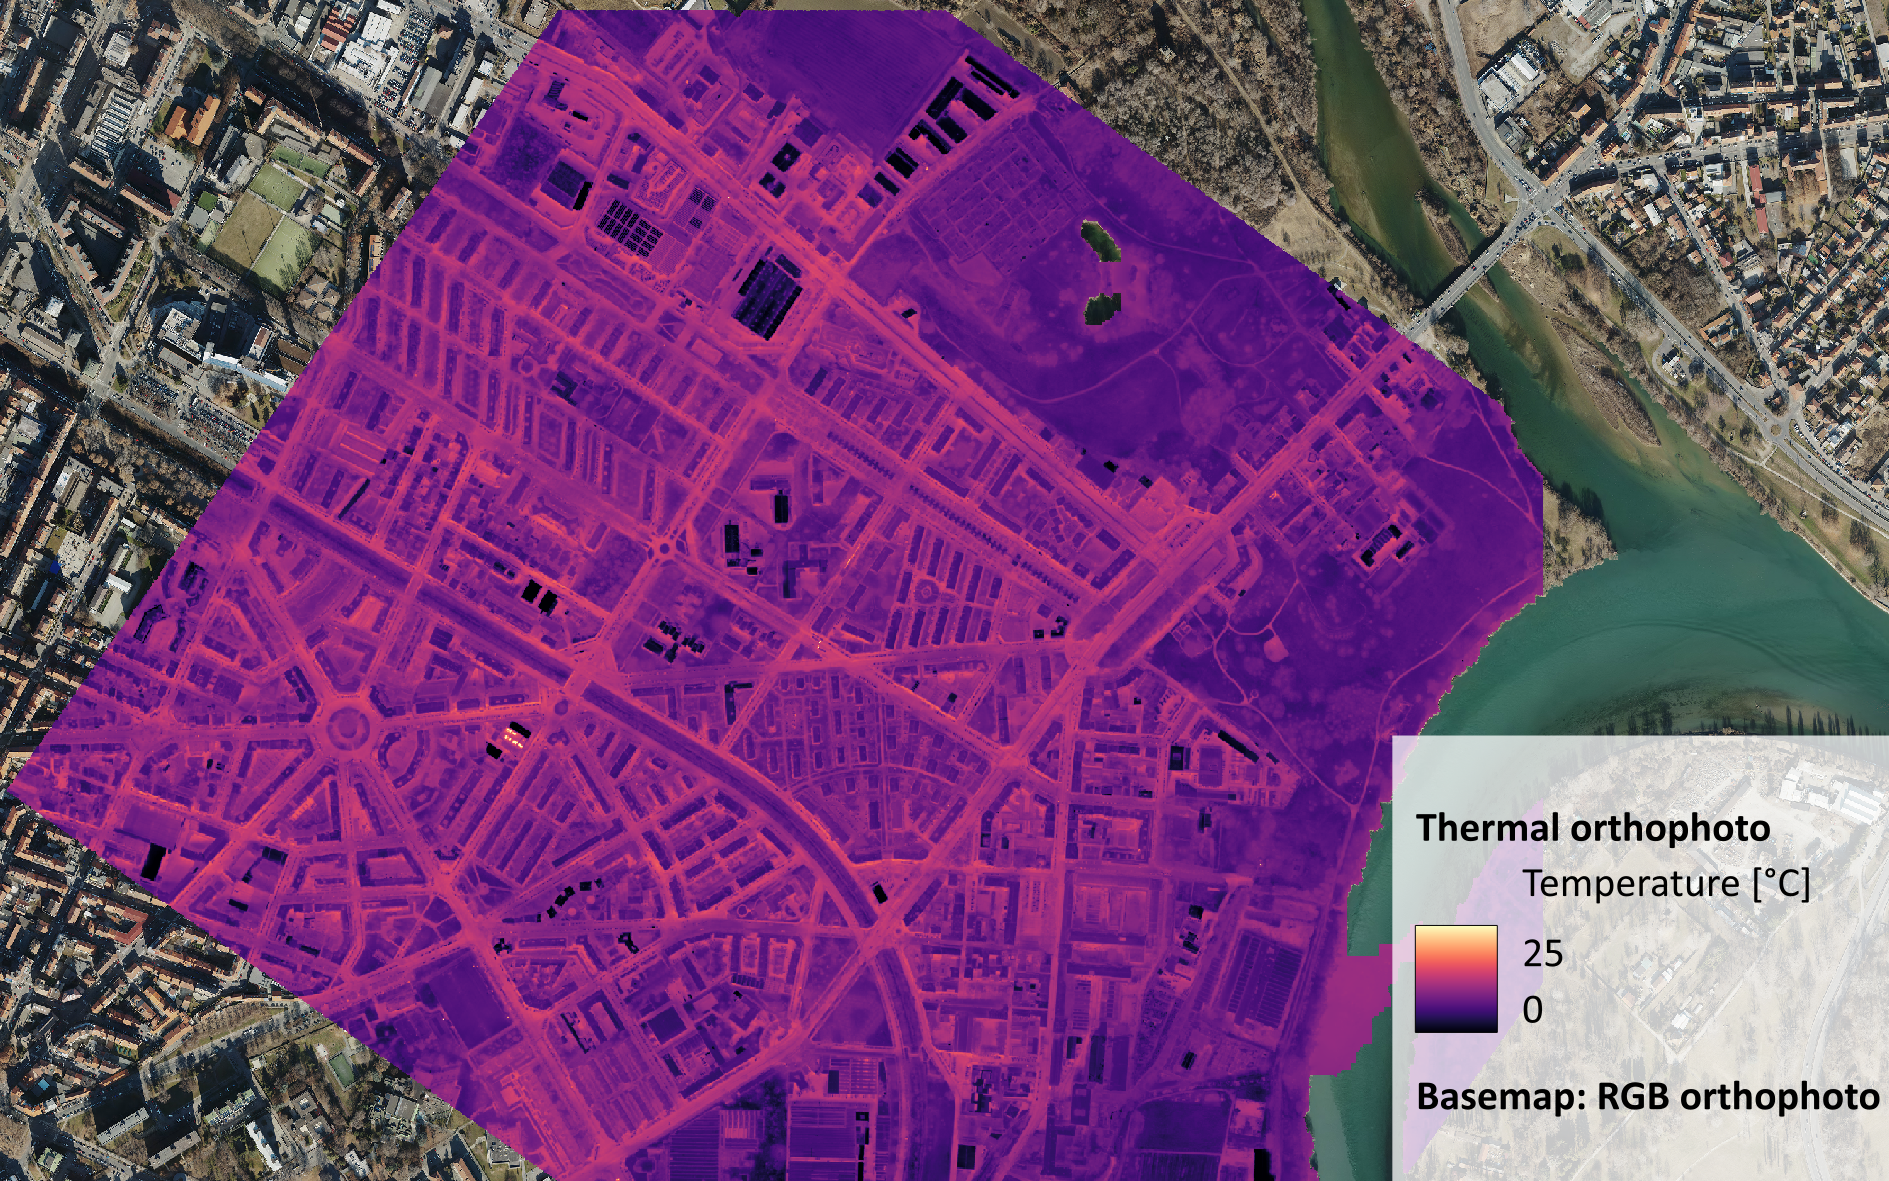
\includegraphics[height=0.5\linewidth]{img/Thermographic picture_legend.png}
            \caption{Thermal image overlayed on top of Turin orthophoto (thermal image overlay on top of aerial photo within the visible light range.}
            \label{fig:therm-ortho}
    \end{figure}
        
    \subsection{Machine Learning in Energy Usage Intensity Prediction}%CLC
        Using machine learning (ML) to predict EUI is no longer a new concept. A set of 49000 EPCs was used to define a benchmark for building energy performance, resulting in a RMSE equal to 44.47 and a MAE equal to 30.54\cite{piscitelli_interpretable_2025}. Wider dataset were also used in stattistical approaches, as in the case of Milan, with more than 200000 EPCs used\cite{mutani_statistical_2023}. Energy Usage Intensity, known as energy consumption per unit floor area\cite{energystar_energy_2014}, often sees itself reported with a unit of `kWh/$m^2$/year` as an annual value. Unlike more traditional EUI prediction methods which heavily rely on heat-transfer-based modeling and statistical regression on known data that requires significant amount of prior knowledge on the topic to make sense of the results, ML algorithms are much easier to be use and much more straightforward to generalize\cite{amasyali_review_2018}. Unlike the traditional approaches, ML algorithms require much less abstraction and can capture complex, non-linear relationships between different input features (from building envelope to system type, numerical to categorical) and building energy consumption, enabling more accurate and generalizable EUI predicitons\cite{seyedzadeh_machine_2018}. 
        
        Regarding the types of ML models that researchers have used in predicting EUI values, aside from simple linear/logistic regressions, algorithms such as artificial neural networks (ANNs), support vector machines (SVMs), decision tress and ensemble methods\cite{ahmad_building_2016,wang_novel_2018} also saw their place in the existing literature lineup. ML algorithms, regardless the actual alternative model that was selected, learn a series of parameters that fit a model that best predict the energy consumption data within the historical energy consumption profile reserved for training\cite{deb_review_2017}. Performance of these models obviously relies on how good and representative the training data is compared to the test set (or more importantly when put into test as a real use case)\cite{jain_forecasting_2014,touzani_gradient_2018}. More recently we have seen studies that advances more towards deep learning models, particularly with convolutional neural networks (CNNs) alongside recurrent neural networks (RNNs)\cite{fan_short-term_2017,li_buildings_2015} with promising results.

        As the parameters are clearly trained out from the dataset provided, like all ML use cases the first challenge in using ML to predict EUI is overfitting. If the dataset provided is not large/representative enough, regardless how much effort is put into the modeling process, the resulting model that predicts the building EUI will still perform poorly out-of-sample data\cite{amasyali_review_2018,seyedzadeh_machine_2018}. Alternatively, cross-over researchers also tend to face challenges in appropriate feature selection process and hyper-parameter tuning\cite{touzani_gradient_2018} when fitting/finetuning their models. Moreover, it is worth noting that the more complex the model, the less interpretable it becomes. For multiple-tree models like gradient boosting regressor, the interpret-ability is already bad enough, but when facing models like neural nets, there is simply no easy way to illustrate the reasoning process of the model other than a graph theory network\cite{wang_novel_2018}. This lack of transparency is one clear aspect that limits further implementation of ML in predicting EUIs.
        
    \subsection{Knowledge Gap}%CLC
        Despite both being used heavily in the building sector right now, thermal imaging and machine learning have seen little joined investigation that attempts to set up synergy between the two methodologies. To begin with, there is an absence of large-scale, high-quality datasets that have both thermal imagery and associated building energy consumption data that would enable any ML investigation\cite{amasyali_review_2018}. Hence, there are also currently no clear attempts on extracting relevant features of building-footprint-related thermal imagery features from raster files. On a similar note, there will hence be no existing studies that discuss how to best conduct investigation on how to engineer additional features for ML based off the building-specific thermal information rom the raster data. These knowledge gap highlights the need for our proposed research where we will attempt to set up an effective fusion of both techniques as an exploration at their intersection.  

        We do want to acknowledge the limitations that an investigation will likely face ahead of going into our methodology. To begin with, despite claiming that our approach will excel in scalability and generalizability, our model will be specific only to the building type\cite{ahmad_building_2016} and urban landscape \cite{jain_forecasting_2014} and the current climate zone. As we previously mentioned regarding the emitted radiant heat from surfaces, even with the same surface material, a constantly dry surface will have a different effective emissivity in comparison to a surface that is consistently wet surface, e.g. Abu Dhabi vs. Singapore. We will try to set up a ML pipeline that is blind to region-climate specific tuning as it only leverages thermal images. That said, recognizing the challenges posed by emissivity will see itself embedded in the thermal images themselves, the ML pipeline will need to be well-designed to circumvent this effect as much as possible.
        
\section{Methodology}%CLC
     We present our methodology in this section describing details regarding how we collected, preprocessed and merged our data for machine learning, and how we tackled alignment issues between the EPC data (tabular) and thermal imagery (raster) data. Our proposed approach involves both the energy performance certificate data and the thermal image that we collected, putting them through pre-processing to remove the null values and outliers, spatially joining the two together, and obtaining the corresponding dataset for the modeling stage to go through feature engineering, selection and alternative model selection before coming up with a trained model that allows for leveraging thermal-imagery-based-features only to generate EUI predictions. We have created a diagram that illustrates how these different components come together within our methodology in Figure \ref{fig:roadmap-diagram}. In this flow chart we provide a concise overview of the entire workflow of the current study, with more detailed breakdown of additional steps in subsequent figures and illustrations.
     
    \begin{figure}[h!]
        \centering
        % 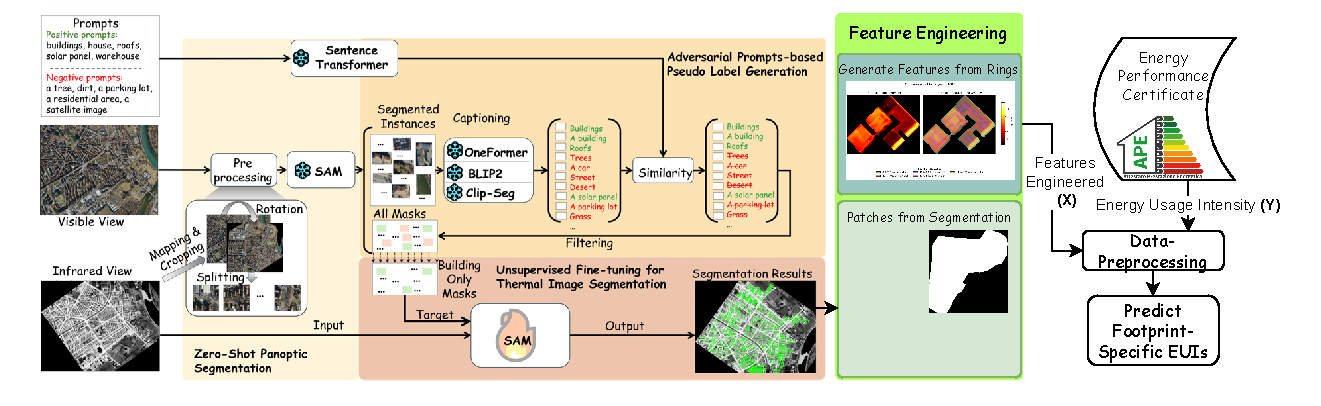
\includegraphics{img/SegmentWorkflow.pdf}
        \includegraphics[width=0.95\linewidth]{img/Segment.png}
        \caption{Overall Methodology WorkFlow: From Data acquisition to preprocessing thermal image and obtaining modeling targets via EUIs through EPC and creating Auto-ML-enabled Regression.}
        \label{fig:roadmap-diagram}
    \end{figure}


\subsection{Study Area}%CLC
    The investigated area is located in Turin, Italy, a medium-sized city in North-West Italy, at the foot of the Alps. The 2$km^2$ study area, part of the Barriera di Milano neighborhood, is characterized by buildings constructed quickly and poorly in the post-war period (as is shown in Figure~\ref{fig:enter-label}) to accommodate the city's 40\% population increase \cite{ISTAT2024}. The continuous marginality conditions of its population have led to a state of physical degradation and inadequate energy performance.

    \begin{figure}[h!]
        \centering
        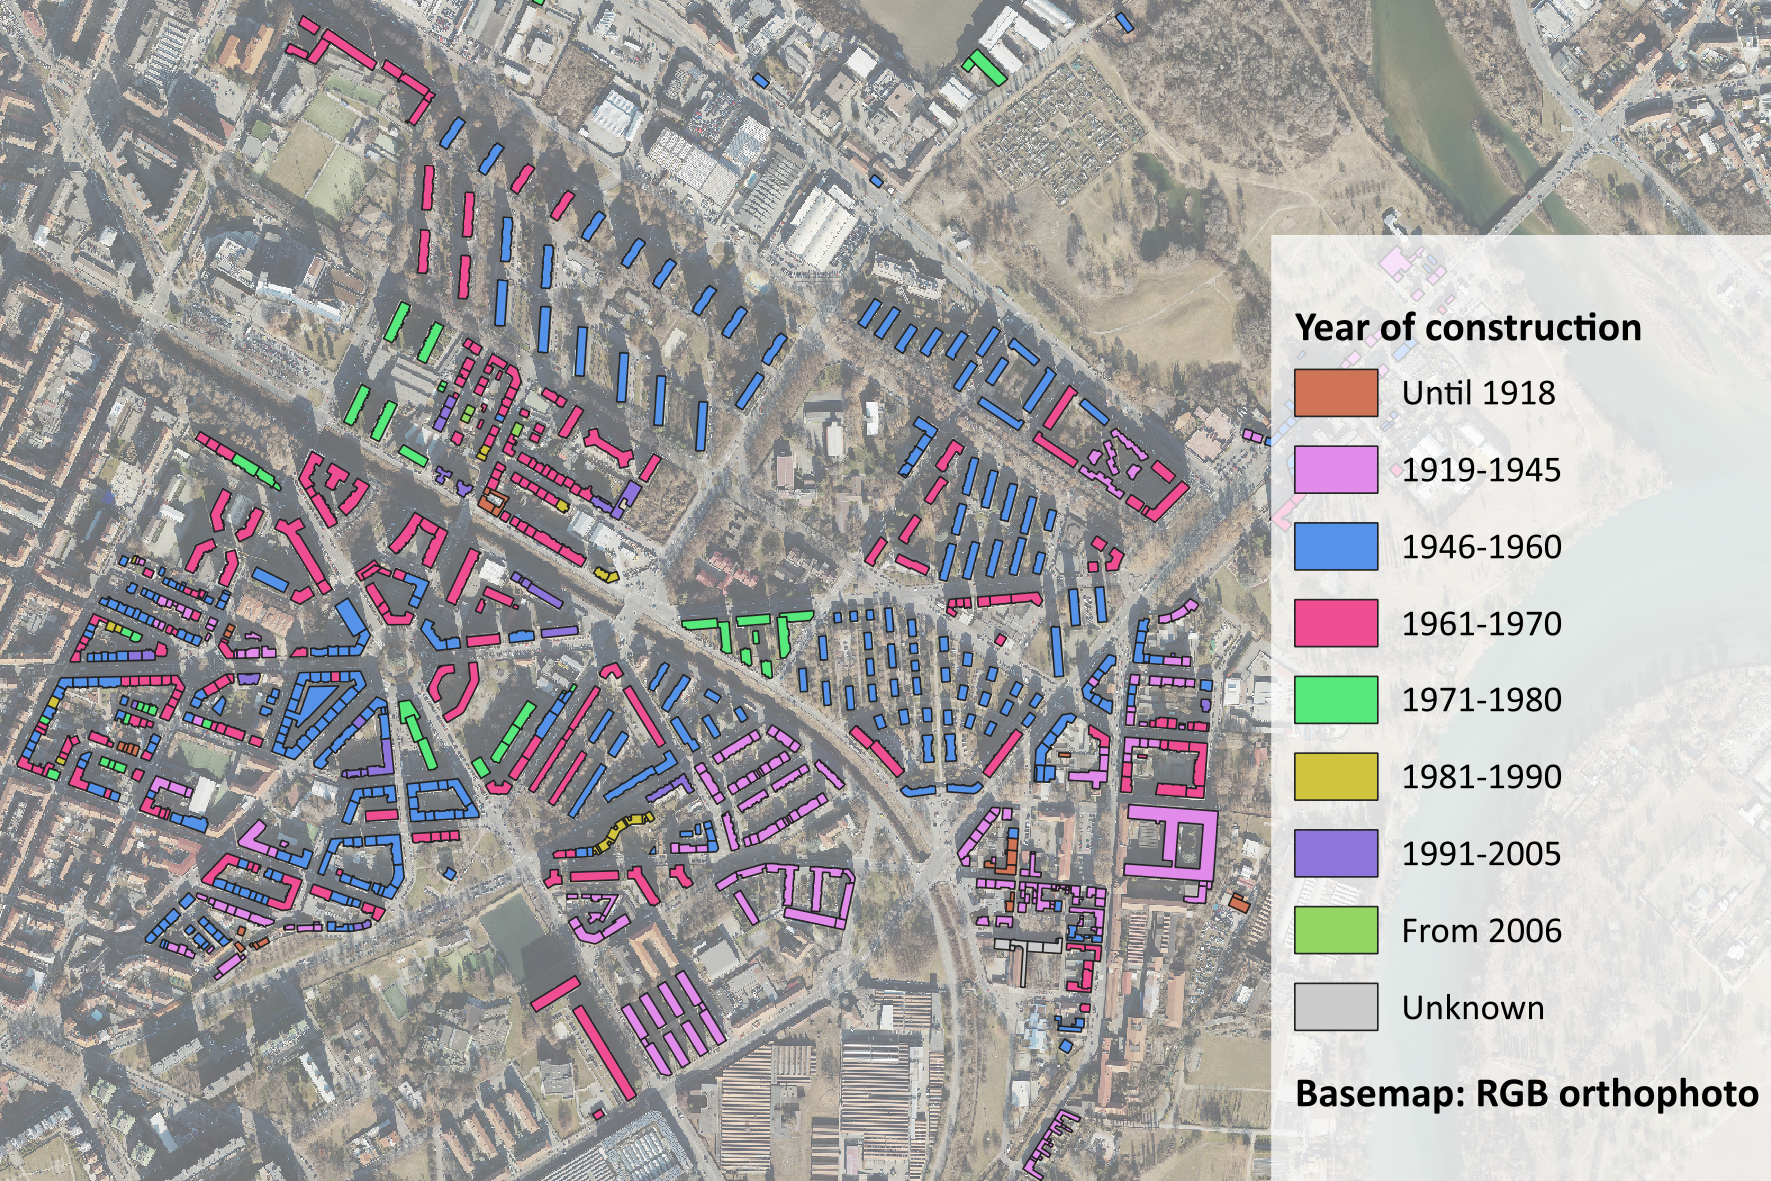
\includegraphics[width=0.85\linewidth]{img/Year of construction2.png}
        \caption{Site investigated by the thermal imagery colored by time of construction in buckets in Turin, Italy.}
        \label{fig:enter-label}
    \end{figure}
    
    The study area's urban morphology and construction year highlight some homogeneous areas. The former railway trench, built in the XIX century and abandoned in 1990s, acts as an edge between the historical town in the South and planned districts in the North. Two social housing districts, Taranto Avenue and Gottardo Street, were realized starting from 1946, consisting of sixteen eight-floor and ten three-floor buildings, respectively\cite{Comoli1984}. In contrast, the Southern part, around Respighi Square, evolved organically with smaller volumetric units and varying heights.

    Turin's weather and environmental conditions further emphasize the need for extensive renovation in the aging building stock. The city experiences increasingly hot summers and freezing winters, resulting in high demand for both heating and cooling. In the period 2014-2023, Heating Degree Days and Cooling Degree Days were 2587 and 85, respectively \cite{Agri4CAST}. In particular, in 2023, in 26 days temperatures below 0$\degree C$ were registered and the average temperatures in January and February were 2.0$\degree C$ and 4.2 $\degree C$ – respectively. On the other hand, 2023 has been the second hottest year since 1958, with 64 days in which temperatures exceeded 30$\degree C$. These extreme temperature variations can lead to a wide range of EUIs across the building stock, depending on the thermal performance of the envelope and the efficiency of the HVAC systems.
    
    Meanwhile, buildings with poor insulation and outdated heating and cooling systems are likely to have higher EUIs compared to those with more efficient and well-maintained systems. There's also a tendency towards conditions enhancing air pollution, such as negligible wind gusts (1.7 m/s on average) and decreasing rainfalls (8\% deficiency compared to 1991-2020 averages) \cite{ClimateARPA}, leads to high concentrations of pollutants like PM10, exceeding the European legislation threshold \cite{EuropDirective}. These environmental factors can further influence the energy consumption patterns of buildings, as occupants may rely more heavily on mechanical ventilation and air conditioning systems to maintain indoor air quality and thermal comfort.

    Energy classification is a first step for defining priorities in refurbishing the ageing building stock, thus favoring the increase in the sustainability of the building stock and of the city as a whole. The interest of the Municipality is to foster energy renovation and transition starting from the outskirts, in order to reduce inequalities and add value to downgraded areas. From this, in accordance with the Public Administration, it was decided to focus on the area of \textit{Barriera di Milano}.


    The selected study area in Turin represents a challenging and diverse urban environment that can greatly benefit from energy usage prediction (by association potential energy classification) and retrofitting initiatives. Its mix of historical and post-war buildings, varying urban morphologies, and critical weather conditions make it an ideal testbed for evaluating the effectiveness of our proposed methodology in promoting energy efficiency and sustainability in complex urban contexts.


\subsection{Data Acquisition}
    \subsubsection{Thermal Image}\label{sec:therm}%CLC
        The acquisition of the thermal picture was performed on $23^{rd}$ March, 2023, from 6 pm to 8 pm, after sunset. The nighttime acquisition was preferred as it makes it possible not to perform any correction of potential biases emerging from solar radiation. In order to compare similar objects - buildings in this specific case - observing the relative temperature differences rather than the absolute temperature value, it was chosen to use a thermal camera registering midwave infrared bands, from 3 $\mu m$ to 5 $\mu m$, that is the FLIR A8581 MWIR HD. Midwave infrared cameras ensure higher spatial resolutions, resulting in a Ground Sampling Distance equal to 20 cm. This allows proper modelling of the building, minimizing the risk of the mixed-pixel bias, i.e. the error resulting from the inclusion in the same pixel of surfaces pertaining to different entities. Indeed, high resolution allows for a good separation between buildings and neighboring elements in the orthoprojection. The acquisition, with a ±1°C accuracy, was performed over an area of approximately 2 $km^2$, covering a surface including both buildings and urban parks, in particular the two along the Stura and Po rivers, in the North and East respectively, as shown in Figure~\ref{fig:therm-ortho}.
        

    \subsubsection{EPC dataset}

    The Sistema Informativo sugli Attestati di Prestazione Energetica (SIAPE) is Italy's central database for Energy Performance Certificates (EPCs), overseen by ENEA, the National Body for New Technologies, Energy, and Sustainable Economic Development\cite{lavecchia_predicting_2024}. Established to support the country’s commitment to the EU’s Energy Performance of Buildings Directive (EPBD)\cite{gatt_assessment_2020}, the database collects detailed information about the energy efficiency of buildings sold, rented, or significantly refurbished since 2010. However, it currently provides EPC data in aggregated forms, from national down to provincial levels, which can limit detailed site-specific analysis. 
    Although the SIAPE contains approximately 7.2 million records, its coverage is nearly comprehensive across Italy, with the primary exception being the region of Sardinia.
    In Piedmont region, disaggregated EPC data are accessible through the regional open data portal known as datipiemonte. Contrary to the SIAPE, the platform provides all EPC data in a disaggregated format, which can be crucial for conducting site-specific energy analysis and research. It is worth noticing that within the scope of this study, EPC data are solely used to obtain EUIs and to associate each thermal image segment with its corresponding geographic location. We do not use EPC data to derive additional predictive features or to enhance data quality; instead, they serve as the ground truth benchmark for our thermal imagery-based prediction models. The results that we obtained are, therefore, also not leveraged to enrich the EPC data or fill missing its missing values either.
    
    However, these data are provided separately, in various individual tables and sections that need to be cleaned, organized and potentially aggregated for our proposed usage: create energy usage profile (i.e. EUIs) of building blocks. Given these complexities, we recognize the need for substantial data transformation, which includes merging datasets by shared indices and using geospatial analysis to connect the information accurately. By transforming and integrating these datasets, we aim to improve building energy efficiency evaluations, supporting smarter urban planning and aligning with both regional and national energy goals.
    
   
\subsection{Data Processing}
    \subsubsection{Challenges in Thermal Image Resolution for Segmentation}\label{seg:thermnum}%CLC
    Upon researching relevant approaches, we noticed that currently there has been very little effort to segment thermal images despite an abundance of existing body of research on segmentation \cite{kirillov_segment_2023} that allows for segmentation of building footprints from satellite images, resulting in not only methodologies but also publicly available datasets \cite{microsoft_microsoftglobalmlbuildingfootprints_2024}. Upon reviewing the methodologies, we believe this could be attributed to the mismatch of thermal image resolutions in comparison to high-resolution optical (e.g., RGB) aerial or satellite images: images that have been used to train the segmentation models usually have a much better resolution. The thermal infrared satellite imagery (such as the one provided by Sentinel 3 or Landsat) has coarser resolutions in comparison to remotely-sensed pictures acquired in different bands, with the ground sampling distance being from 30 m to 100 m on average, contrary to RGB bands with resolutions up to few centimeters. To put it into perspective, the visible spectrum extended from about 0.4 $\mu m$ (violet) to 0.7 $\mu m$ (red), and the infrared spans between 0.7 to up to several hundreds $\mu m$. As the speed of light $c=\lambda v$ dictates, the longer the wavelength, the smaller the frequency of light, which timed by the Planck constant gives us the energy of light to its current frequency. On that front, the energy that a remote sensing device acquire will naturally be much harder as the sensor increases its instantaneous field of view (IFOV) to cover larger areas to get enough energy to make reliable measurement. For this very reason, the resulting range of imagery had an obvious mismatch between the thermal and the image within the visible light range as shown in Figure ~\ref{fig:therm-ortho}.

    %HERE WE INITIALLY HAD THE MSFT FOOTPRINT BUT DELETING AS IT NO LONGER EXISTS.
    % Noticing the challenges in our initial attempt, we went ahead and leveraged the aforementioned dataset from Microsoft \cite{microsoft_microsoftglobalmlbuildingfootprints_2024} for more reliable groundtruth of segmentation as shown in Figure \ref{fig:footprint-overlay}. This allowed us to test various alternatives between zero-shot learning and few-short learning for finetuning to a best-performing modeling pipeline.
    % \begin{figure}
    %     \centering
    %     \includegraphics[width=0.5\linewidth]{img/overlay_footprint.png}
    %     \caption{Overlay of footprints from MSFT, satellite image and thermal image.}
    %     \label{fig:footprint-overlay}
    % \end{figure}

    The refreshed pipeline of segmentation allowed us to generate the coordinates on the thermal images that allowed us to cut the thermal image into small segments that can be further batch processed into location-based features that can be joined to the unit-specific EPC datasets to test their predictive power for the energy usage intensities. We first extracted obvious features from the thermal images, this includes key statistical metrics, including mean, median, minimum and maximum temperatures as well as specific percentiles to capture the granular view of temperature distribution.
    
    
    \subsubsection{Preprocessing of EPC dataset}%CLC
        Committing to the promises it made in Paris Agreement, the EU requires EPC for each built property among EU nations whenever there is a new building that requires any government-funding or is listed for resale/rental. The EPC data used in this research are collected by Italian National Agency for the Technologies, Energy and Sustainable Development (ENEA). The open data portal of the Piedmont Region allows for the public access to the collected, raw EPC data for Piedmont region, allowing access to 
        a total of 7 tables, which upon further examination had varying data availability within: 
        the majority of the relevant information that we need resides in the first four tables (covering aspects like building systems, energy consumption, and property details), key statistics for which are outlined in the following Table~\ref{tab:transposed_table_stats}. 
        Recognizing the curse of dimensionality as the number of columns combined within the top 4 tables mounts up to 242, we decided to only leverage the top 4 tables out of the 11 tables inside the dataset due to missing data entries for merging including crucial information such as latitude, longitude, etc. This allowed us to pull relevant records within all four tables for the city of Turin within the cadastral sheet numbers of [1085, 1098, 1099, 1100, 1102, 1131, 1132, 1133, 1143, 1144, 1145, 1146, 1147, 1148, 1188, 1189], which allowed us to pull all relevant records for further data-cleaning and got to a subset of records whose data availability quickly drops from up to 81\% to below 40\% as we are showing in Table~\ref{tab:transposed_table_stats}.
    
       \begin{table}[h!]
        \centering
        \resizebox{\textwidth}{!}{%
        \begin{tabular}{|l|c|c|c|c|}
        \hline
        \rowcolor{gray!30} \textbf{Statistic} & \textbf{Systems} & \textbf{Recommendations} & \textbf{Consumptions} & \textbf{Details} \\ \hline
        Number of Rows           & 13,155  & 7,093  & 10,849  & 6,588   \\ \hline
        Number of Columns        & 55      & 55     & 53      & 79      \\ \hline
        \% Columns Filled $\geq$ 80\% & 78.18\% & 81.82\% & 79.25\% & 37.97\% \\ \hline
        \end{tabular}%
        }
        \caption{Transposed Summary Statistics for Selected Tables}
        \label{tab:transposed_table_stats}
        \end{table}
        
        Leveraging the understanding towards the data availability, we were able to combine the four tables by creating a unique identifier across them, recognizing the fact that each unique EPC record ID could be associated with different properties. With this step we are able to create relationship across tables that were inherently connected but without explicit relationship ID. We constructed the unique key by stitching the EPC record ID with the detailed address (street name and house number). This allowed us to obtain ultimately a record of approximately 4000 unique EPC records, each with with more than 200 columns (after dropping duplicates such as latitude/longtitude, etc.) within the identified region in Turin for further processing. It is important to clarify our decision to use Energy Usage Intensity (EUI) rather than Primary Energy (PE) as the prediction target. While PE is readily available in EPC datasets, EUI provides a direct representation of the actual energy consumed per unit floor area, making it more intuitively interpretable for urban planners and policymakers when evaluating retrofit potential. Furthermore, using EUI aligns better with common international practices and allows our methodology to remain consistent and broadly applicable across different regional energy policy contexts.

    
       \begin{figure}[h]
            \centering
            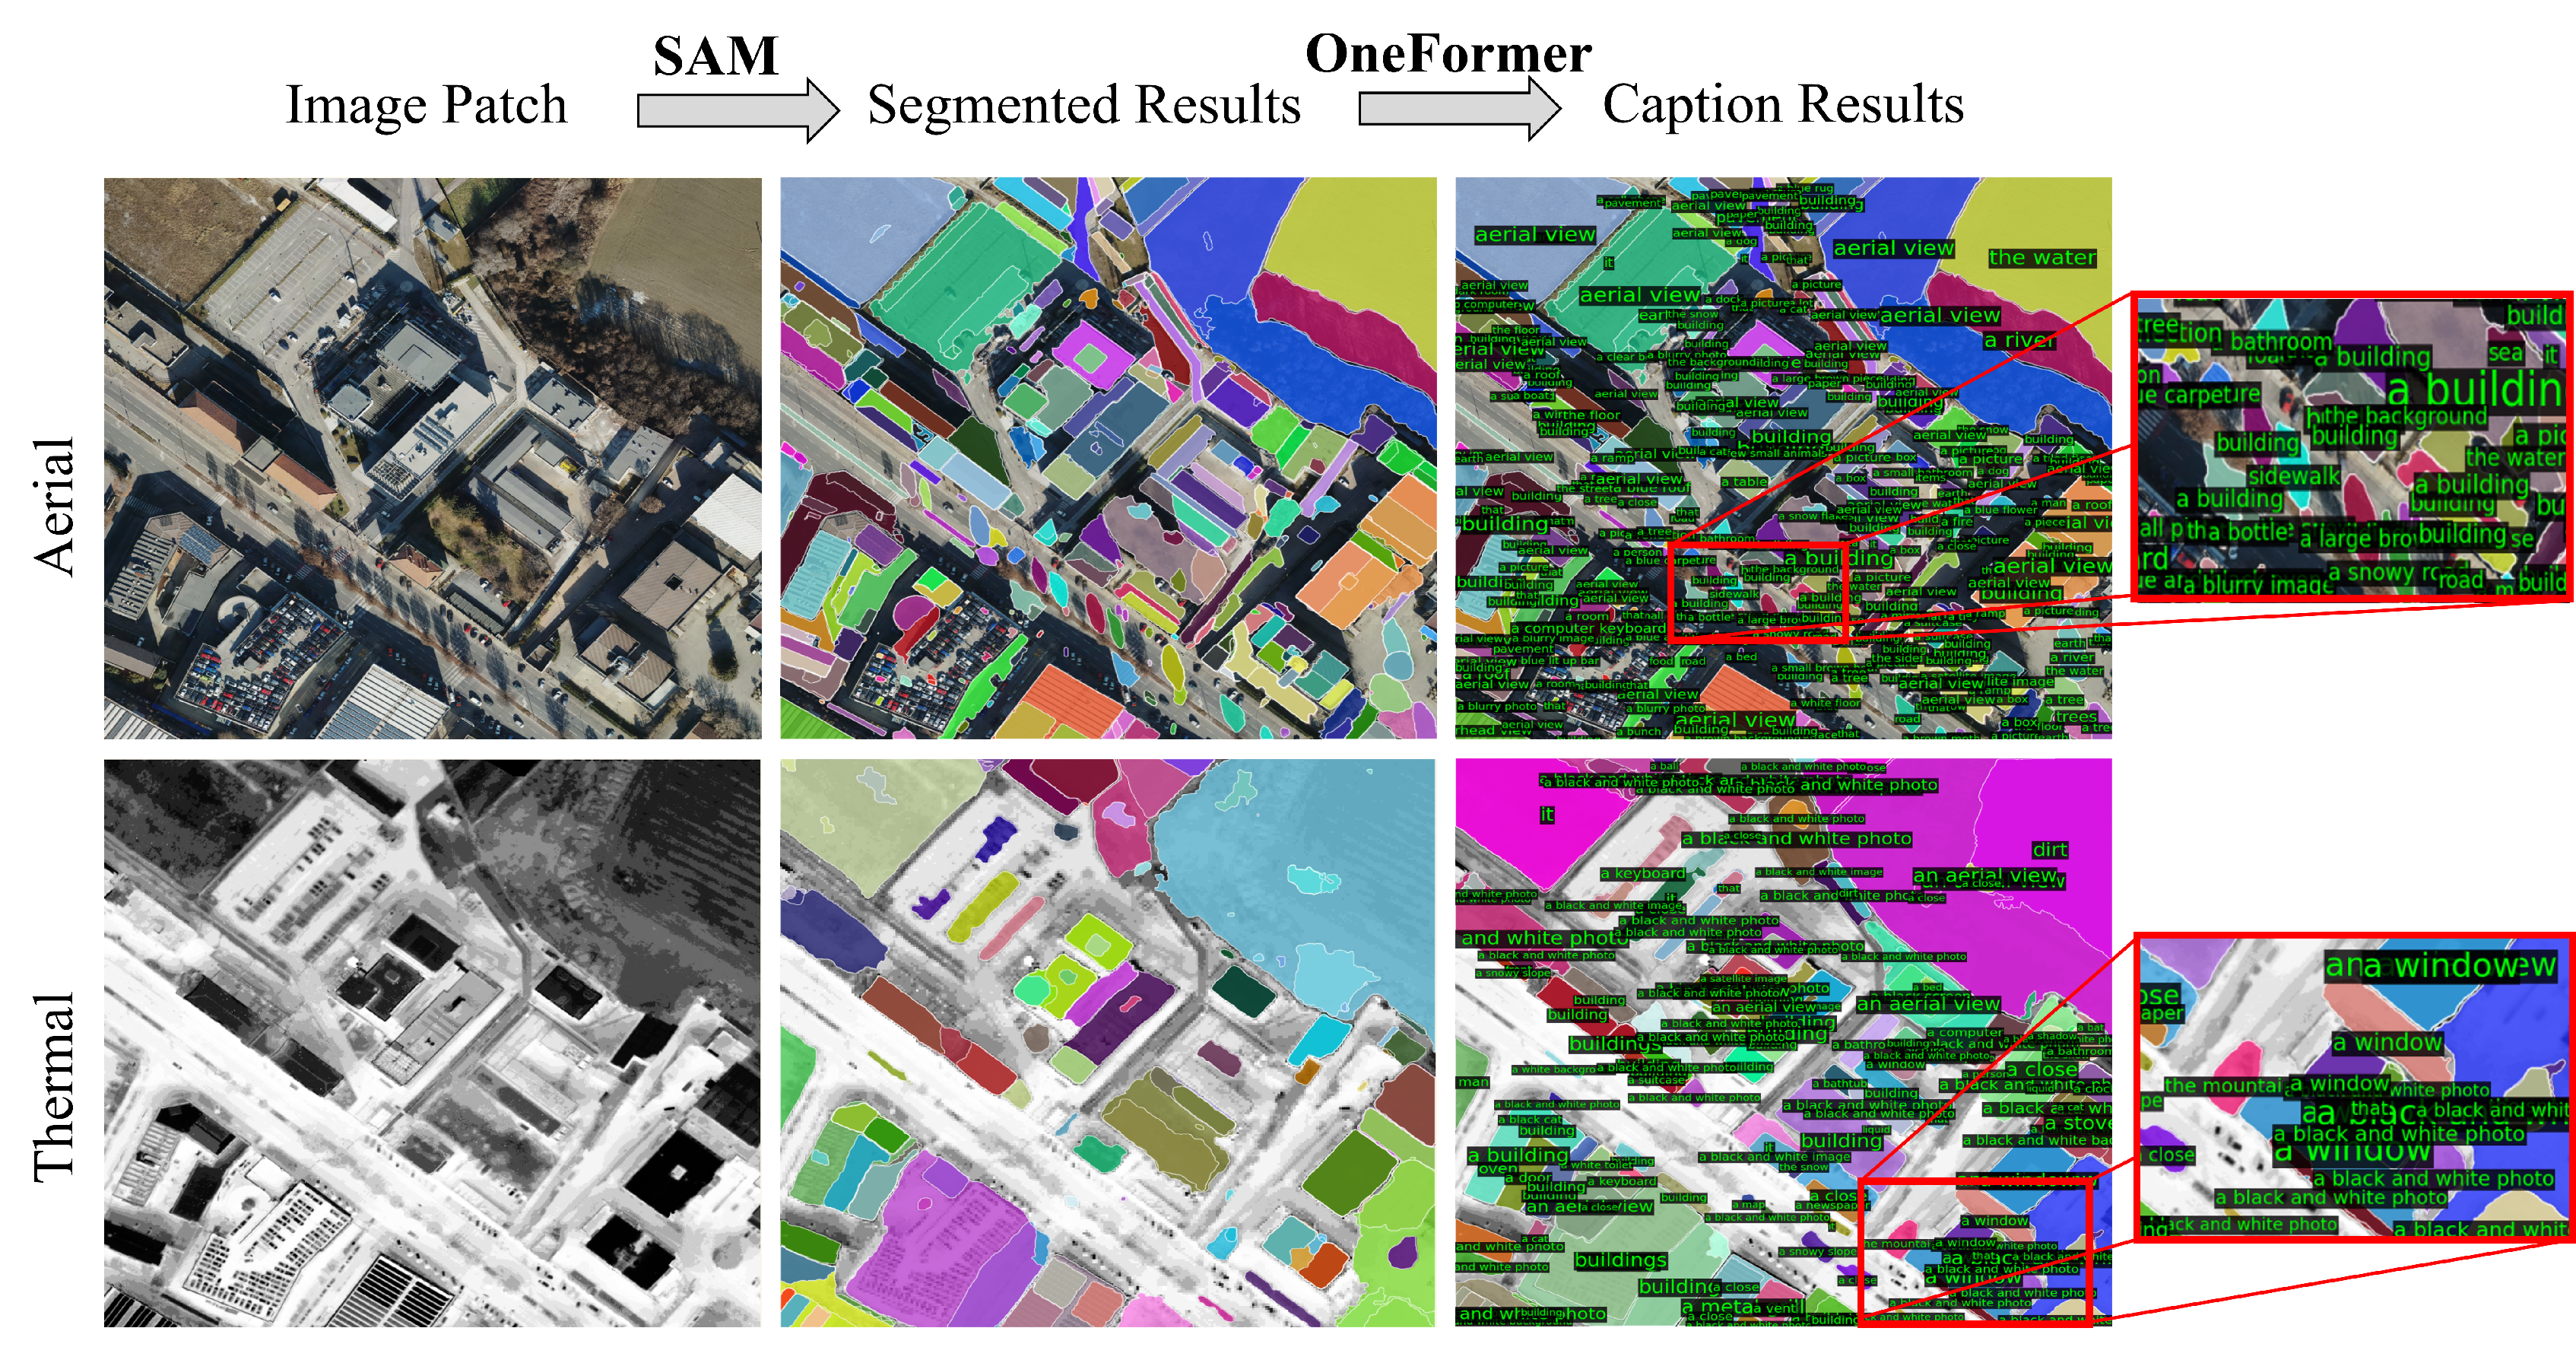
\includegraphics[height=0.47\linewidth]{img/challege.pdf}
            \caption{Thermal image segmentation challenges: Unrelated object, wrong segmentation, wrong labels ...}
            \label{fig:thermseg-challenge}
        \end{figure}
    
    \subsubsection{Unsupervised Thermal Image Segmentation Pipeline}
        As our prior art search revealed, there has been very little effort within the research community to address the segmentation of thermal images with computer vision  due to the mismatch of resolution - which is inevitable due to how thermal information has a much lower level of energy that can be captured by the same lens as with visible light. A good example of how that looks like can be found also in Figure~\ref{fig:therm-ortho} - the coverage of thermal image was only about 1/4 of the overall range of visible light collection. Recognizing the better-resolution-ed underlying city terrain, we decided to develop a two-pronged approach that allows us to leverage the underlying image for segmentation footprint, and then cut out the actual building patch from the thermal image with these explicit coordinates.


       \begin{figure}[h]
            \centering
            \includegraphics[height=0.55\linewidth]{img/workflow_n.pdf}
            \caption{Thermal image segmentation workflow.}
            \label{fig:thermseg-workflow}
        \end{figure}

    Figure~\ref{fig:thermseg-workflow} illustrates our unsupervised thermal image segmentation pipeline, which comprises three processing stages. This pipeline generates thermal image patches that are extracted from the full thermal image shown in Figure~\ref{fig:therm-ortho}.
    
    In the first stage, we integrate aerial imagery as a base map for initial processing. The aerial image in the visible light range corresponding to the thermal image is divided into smaller patches, with the patch size determined by the spatial coverage of the pre-trained model. Each patch is then processed to produce instance segmentation for various objects (e.g., buildings, pedestrians, cars).
    
    In the second stage, we incorporate an image captioning module composed of OneFormer \cite{jain2023oneformer}, BLIP2 \cite{li2023blip}, CLIP-Segment \cite{luddecke2022image}, and Sentence Transformer \cite{reimers2019sentence}. Each segmented object from SAM is initially assigned a coarse-grained label using OneFormer and subsequently enriched with fine-grained details via textual captions generated by BLIP2. To determine the final label for each patch, the CLIP-Segment model selects the label with the highest segmentation confidence from the enriched captions. Given that our primary interest is in building-related objects, we apply an additional filtering layer using a sentence transformer with positive prompts (associated with buildings) and negative prompts (associated with non-building objects). This filtering step retains only the objects identified as buildings while excluding irrelevant elements such as streets, cars, and vegetation. The coordinates of the identified building segments are then used to extract the corresponding thermal patches from our measurements. However, due to distortions and variations in geolocation accuracy between the satellite and thermal images, approximately one-quarter of the segmented coordinates do not align perfectly with the thermal images.
    
    In the third stage, we fine-tune the SAM model using the segmented results and the filtered building images over one or two epochs. This fine-tuning enhances the model’s ability to accurately segment thermal images and mitigates the effects of misaligned segmentation. Finally, the fine-tuned SAM is applied to generate thermal image segmentations in regions where the satellite-derived segmentation results are suboptimal. This self-supervised approach is fully scalable and eliminates the need for manual data labeling.
    
       \begin{figure}[h]
            \centering
            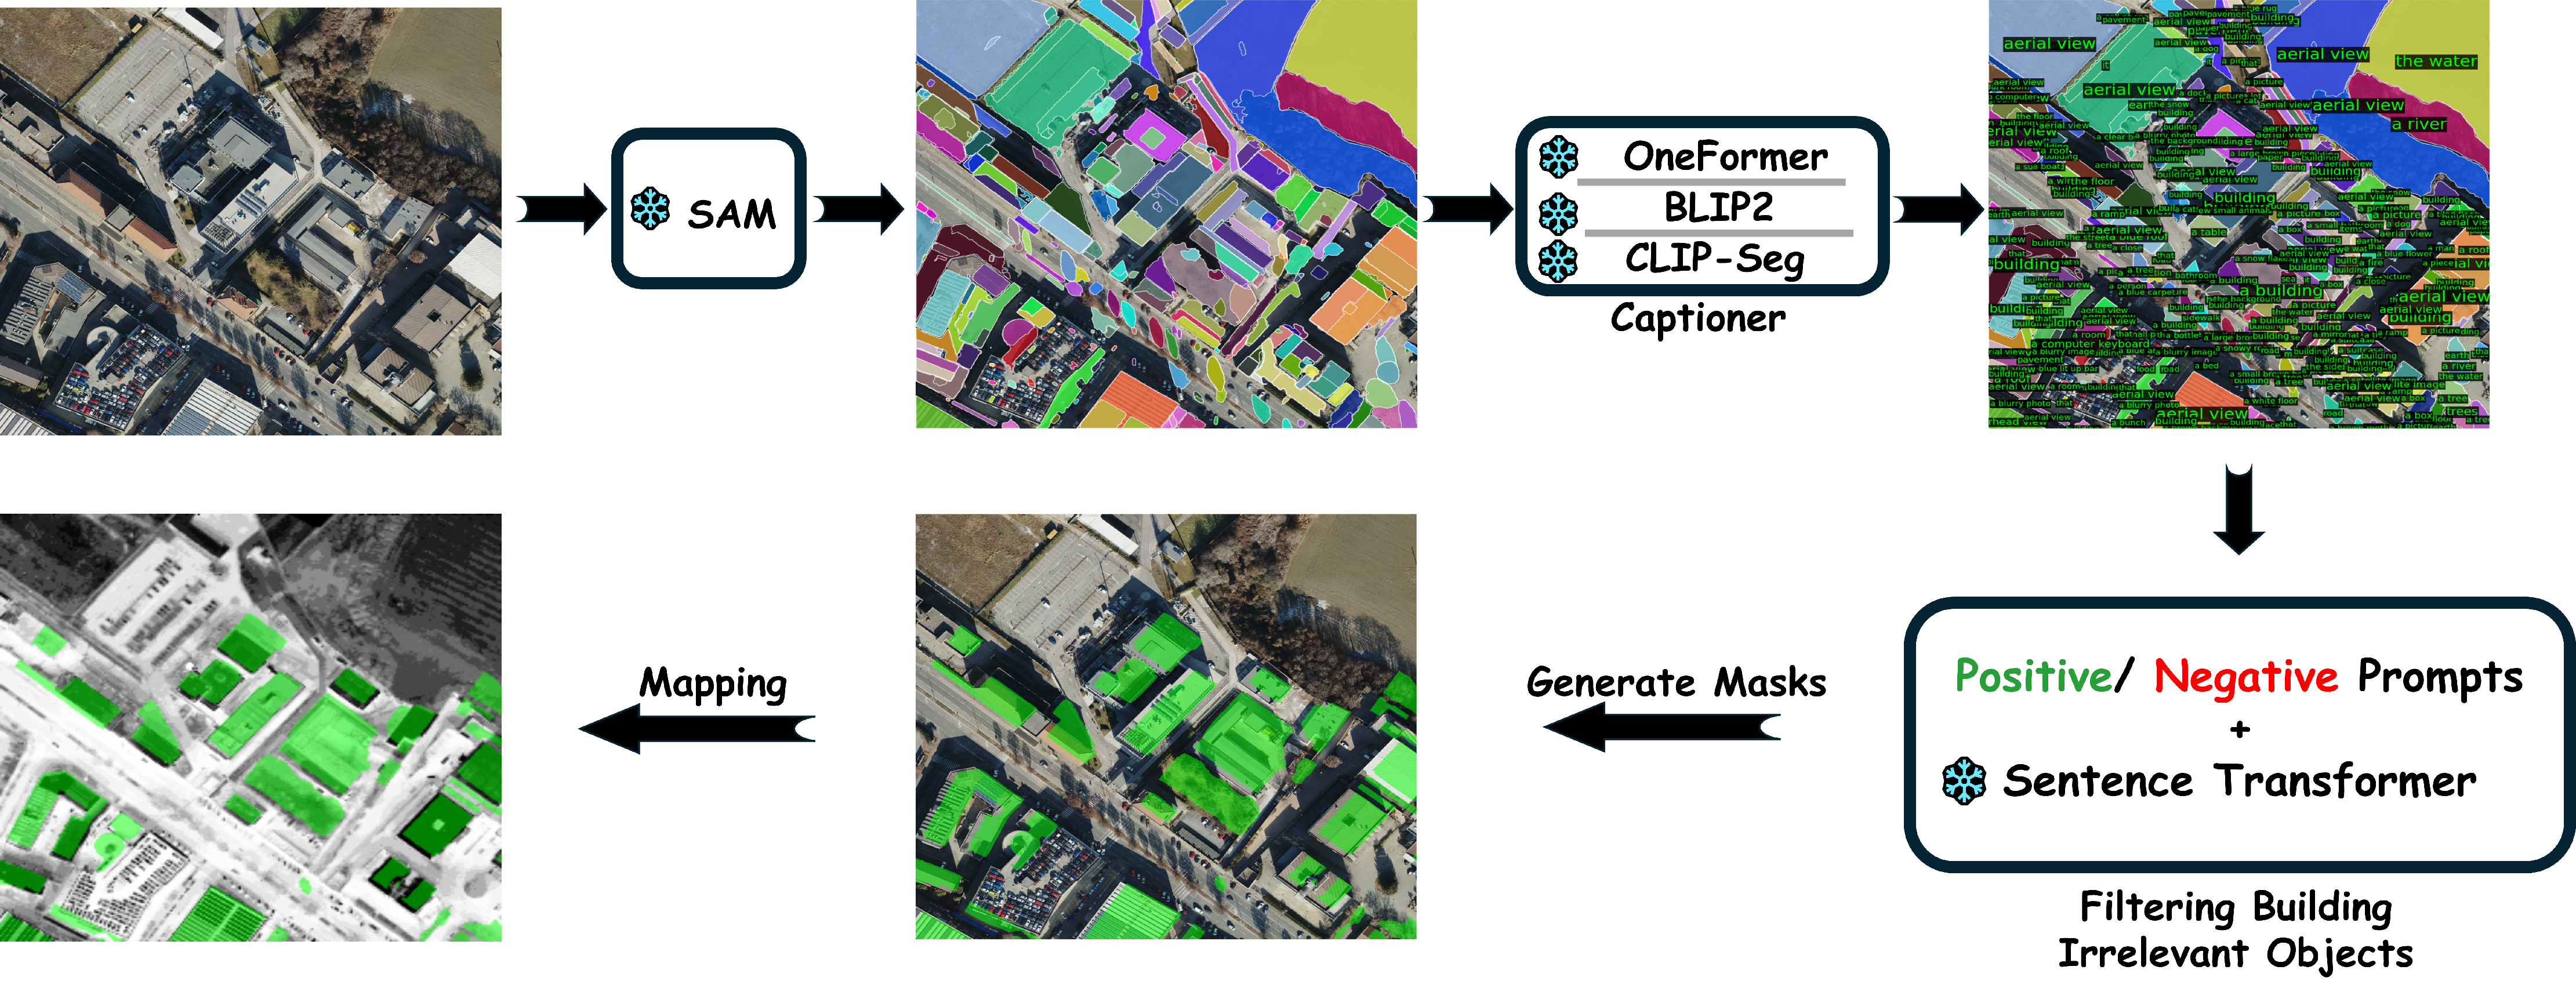
\includegraphics[height=0.4\linewidth]{img/details.pdf}
            \caption{Thermal image segmentation details.}
            \label{fig:thermseg-details}
        \end{figure}

    % (to generate description of how the objects fit together within the patch itself). 
    % As we only want relevant objects that are identified as buildings, we added an additional layer that uses sentence transformer to further process the labeled objects to only keep objects that are identified as buildings, removing streets, cars, grass, etc. The coordinates of the identified building segments are then use to cut out thermal images from our measurements, leading to patches that are most relevant. This self-supervised approach does not require any manual labeling of data, and is completely scalable.
        
   \subsection{Feature Engineering and Selection}%CLC
        It is important to highlight that our methodology exclusively leverages thermal-driven features, explicitly avoiding traditional attributes commonly employed in physics-based or regression-driven EUI prediction methods. Traditional features, such as detailed building envelope properties, occupancy patterns, or HVAC system specifics, often suffer from limited availability, inconsistent quality, and require intensive preprocessing and data cleaning. By contrast, our thermal imagery-based features offer a highly scalable, consistently obtainable, and inherently robust dataset, eliminating reliance on problematic data sources and streamlining large-scale urban energy assessment.
        
        We then proceed to feature engineering, which becomes of a somewhat streamlined process. For each of the segmented patch from our identified footprint, we went ahead and performed a series of extraction, engineering and transformation to engineer features for our EUI prediction. We first calculate the overall stats on the individual patches, namely the mean, max, min, standard deviation, surface temperature values with respect to  every 20\% across the entire temperature distribution on the patch. We then divide the entire patch in to 5 concentric rings (the center-most therefore becomes a polygon). Within each of these ring, the sample statistics are calculated again within each ring for better characterization of the patch identified as we're showing with Figure~\ref{fig:ring-five} with some interesting geometries resulting from the semi-supervised segmentation we conducted. This ring-based approach allowed us to examine how surface temperature variation between the core and the peripheral on the rooftop can have any explanatory power towards EUI prediction. This approach allows us to extract feature directly from surface temperature measurement and convert them into candidates that gets assessed for their predictive powers.

        \begin{figure}[H]
            \centering
            \includegraphics[width=0.65\textwidth]{img/comparison_overlay_38.png}
            \includegraphics[width=0.65\textwidth]{img/comparison_overlay_1002.png}
            \includegraphics[width=0.65\textwidth]{img/comparison_overlay_1010.png}
            \caption{Illustration of patches from segmentation (left) and `rings' of thermal information extracted to be engineered as EUI prediction input features (Patch ID 38(top),1002(middle),1010(bottom))}
            \label{fig:ring-five}
        \end{figure}

        Regarding how we divide these concentric rings, we first define them by radii that incrementally expands outward, effectively dividing the thermal patch into smaller subsets. These subsets will provide valuable information on how the thermal characteristics were like within each of the group, and how the thermal characterizations in both central and peripheral areas. Comparing overall statistics against ring-localized statistics and creating interaction between these columns will also likely result in better model performance. However, as the data that we end up having does not go beyond 1026 rows, the likelihood of our feature engineering process can be further verified outside of these 1026 polygons remains very low. Nonetheless, leveraging these features and adding in additional patch-specific information like the size of the segmentation and the length of segmentation footprint allowed us to arrive at a finalized features' set of 82 columns as input/exogenous features, or for conversation regarding setting up model appropriately, the X or input features for predictive modeling for our prepared dataset. 
        
        % Our investigation here onwards becomes more of a streamlined process, where we treated each of the segmented thermal patches algorithmically to engineer descriptive features on the temperature distribution situation across each of the patches identified. We divided each thermal patch into concentric rings, isolating distinct temperature zones. This ring-based segmentation allows for a targeted examination of temperature variation between the core (rooftop) and the peripheral areas (alongside building envelope), capturing potential thermal gradients and localized temperature anomalies without being over-flooded by general temperature stats.
        
        % Our segmentation approach divides the temperature profile into multiple concentric rings from around the core region. The rings are defined by radii that incrementally expand outward, with each ring representing a specific spatial subset of the thermal profile. For each segmented ring, we calculate the same set of key statistical metrics as we had for the overall image, providing both overall and within-ring thermal characteristics in both central and peripheral areas. We believe our approach provides a structured method to assess temperature distribution across spatial zones, enabling the identification of thermal patterns that might be lost in a global analysis or overshadowed by multi-modal approaches.
        
    \subsubsection{“Derivation of Target: EUIs from Aggregated EPC Data}
        It is worth noting that there is no explicit EUI reported by the original EPC records, pointing to a missing target for our planned usage of the EPC and thermal data. To bridge this gap, a data transformation process was employed to standardize various fuel types and their respective units into numerical values in kWh, leveraging their corresponding conversion factors as we've outlined in Table~\ref{tab:conversion}. Specifically, the quantita\_kwh column was created by mapping specific fuel types and units to their corresponding kWh values, allowing for the efficient conversion of energy consumption data from disparate sources. We opted to use Energy Usage Intensity (EUI) instead of primary energy because EUI is normalized by the building’s floor area, providing a standardized metric that allows for direct comparisons across different building types and sizes; this normalization enables us to extract and compile comparable features for the entire building stock rather than focusing on specific units, thereby facilitating robust benchmarking and analysis of thermal performance at the urban scale.

        It is worth noting that there is no explicit EUI reported by the original EPC records, pointing to a missing target for our planned usage of the EPC and thermal data. To bridge this gap, a data transformation process was employed to standardize various fuel types and their respective units into numerical values in kWh, leveraging their corresponding conversion factors as we've outlined in Table 3.  Specifically, the quantita kwh column was created by mapping specific fuel types and units to their corresponding kWh values, allowing for the efficient conversion of energy consumption data from disparate sources.  We opted to use Energy Usage Intensity (EUI) instead of primary energy because EUI is normalized by the building's floor area, providing a standardized metric that allows for direct comparisons across different building types and sizes; this normalization enables us to extract and compile comparable features for the entire building stock rather than focusing on specific units, thereby facilitating robust benchmarking and analysis of thermal performance at the urban scale.  EPC data are not used directly for prediction but solely to compute the target Energy Usage Intensity (EUI) for each building in our approach.  Due to inherent data quality issues (e.g., incomplete records, use of default values), multiple EPC entries are geospatially matched and aggregated (averaged) to derive a benchmark EUI.  This aggregated target, while imperfect, serves as the sole reference for validating the thermal imagery-based predictions.  This process enabled the calculation of total energy usage consumption, which is a critical input in determining EUI.  Notably, direct kWh values were handled as exceptions, bypassing the conversion factor application altogether.  The 'area' field was calculated by taking the maximum value between the 'heated' and 'cooled area system areas, as both systems contribute to the building's overall thermal load.  Outlier removal and replacement logic was also implemented for fields that do not matter or do not count towards the EUI calculation, ensuring that only relevant data points were included in the analysis.  Although the current model relies on a single thermal snapshot, the methodology is designed to be scalable.  Future work will involve integrating additional case studies with multi-temporal thermal images to capture seasonal variations, thereby refining both the segmentation process and the target derivation.
                
            \begin{table}
            \resizebox{\textwidth}{!}{%
            \begin{tabular}{|l|l|l|}
            \hline
            \textbf{Original Name} & \textbf{English Translation} & \textbf{Conversion Factor to kWh} \\ \hline
            Biomasse solide & Biomass Solid & 9.3 \\ \hline
            GPL & Gasoline & 23.9 Sm$^3$ = 1 barrel, 1 l = 0.001 kWh, 1 kg = 6.52 kWh \\ \hline
            GPL & Gasoline & 11 kg = 1 barrel, 1 l = 0.001 kWh, 1 kg = 11 kWh \\ \hline
            GPL & Gasoline & 6.52 l = 1 barrel, 1 l = 0.001 kWh, 1 kg = 9.17 kWh \\ \hline
            Gas naturale & Natural Gas & 9.54 Sm$^3$ = 1 barrel, 1 Nm$^3$ = 0.001 kWh, 1 kg = 4.78 kWh \\ \hline
            Gas naturale & Natural Gas & 9.54 Nm$^3$ = 1 barrel, 1 l = 0.001 kWh, 1 kg = 9.2 kWh \\ \hline
            Energia elettrica & Electricity & 1 kWh = 1 unit \\ \hline
            Gasolio & Gasoline & 10.2 kg = 1 barrel, 1 l = 0.001 kWh, 1 kg = 10.2 kWh \\ \hline
            Gasolio & Gasoline & 9.17 l = 1 barrel, 1 l = 0.001 kWh, 1 kg = 9.17 kWh \\ \hline
            Solare termico & Solar Thermal & 9.54 Nm$^3$ = 1 barrel, 1 l = 0.001 kWh, 1 kg = 4.78 kWh\\ \hline
            \end{tabular}
            }
            \caption{Conversion table of existing Italian column names of energy type and various conversion factors to be translated to kWh}
            \label{tab:conversion}
            \end{table}

        \paragraph{Why retain EPC--derived EUI targets.} Although as previously outlined a lot of effort was spent on harmonising EPC records---a step that may appear ``merely pre-processing''---those certificates remain the \emph{only} legally mandated, city-wide source of building-level energy‐use‐intensity (EUI) data in the European Union. The Energy Performance of Buildings Directive (EPBD) requires Member States to audit and disclose EUIs whenever a building is sold or leased \citep{EPBD2018_Recast}.  Leveraging this existing infrastructure offers three benefits:
        \begin{itemize}
        \item \emph{First}, predicted EUIs can be compared directly with the energy-class thresholds used by financial-incentive schemes and minimum-performance regulations, enabling an ``apples-to-apples'' retrofit ranking.  
        \item \emph{Second}, the cleaned EPC table released with this study forms a reusable benchmark for future work, filling the data-access gap that often limits cross-city replication \citep{Fabbri2019_EPCreview}.  
        \item \emph{Third}, using EPC-derived EUIs as the \emph{target} while feeding no EPC variables into the \emph{model} provides a stringent test: thermal features alone must explain the variance that EPC assessors normally attribute to construction age, HVAC type, and user behaviour. Hence the pre-processing pipeline is not ancillary but a transferable contribution that bridges remote sensing and policy-relevant metrics.
        \end{itemize}
        

    
    \subsubsection{Spatial Join}%CLC
        With the segmented thermal image patches and the EPC tables joined as one, we are now ready to go ahead and create the dataset that will allow us to test our hypothesis that the introduction of features originating from thermal images will allow us to predict the energy usage intensity of buildings better. 
        We combined the dataset obtained from two streams by identifying a common denominator, the unique, geo-based building ID that is tied to the latitude, longitude and the specific geographical projection system with the geopandas package through a spatial join.%Double check this
        
        From the metadata of the thermal image obtained with airplane fly-over, we understood the 7814 by 6000 pixels image is rendered with a WGS 84 map projection. To best associate our coordinates from the EPC dataset within the thermal image results, we exported the EPC dataset as a shapefile to be joined spatially with the segmented results, allowing us to generate a unique set of building IDs that joins the EPC datasets that are unit-specific to the thermal patches (and their corresponding engineered features) that are geo-location-specific. This is in principle similar to studies that have connected geospatial information to energy usage intensity\cite{lin_using_2017}, some explicitly with disaggregated EUI information\cite{samadi_energy_2021}. Ultimately, this allowed us to compile a record of 1168 EPC records, each enhanced with columns that originates from the thermal patches from our segmentation results.      

    % \subsection{Model Development and Validation}%CLC
    % As we wrapped up the feature engineering bit and went into the modeling phsae, it's important to note that the following section serves more as a record of what we tried that ended up working. Some of the additional work that we ended up doing did not make it to the method section as they were not successful but will get discussed in the Discussions section. From our perspective, as we aim for utmost amount of autonomy from the models, we set up a simple but effective pipeline that does AutoML through PyCaret. Our goal remains the same, where we hope this will unveil how effective thermal-image-based features are in predicting EPC based off calculated EUI values as our label, Y. We performed some basic feature selection in this process to reduce the dimensionality of the dataset by removing highly correlated values that has a Pearson Correlation Coefficient. This not only helped us to achieve reduction of dimensionality, but also mitigated the multicollinearity issues while improving the interpretability of the fitted models. 
    
    % We then modeled upon this dataset with PyCaret. PyCaret is an AutoML framework as we search for the best machine learning model and corresponding hyperparameters that optimizes, in our case, for best EUI prediction. We were able to compare a wide range of ML algorithms ranging from linear regression, decision tress, random forests to gradient boosting machines without having to manually tuning each model. We used this package to help us expedite our modeling process, as the framework itself already automated the data preprocessing, model training, hyperparameter optimization and model evaluation. We then proceed to compare the performance of the models with criteria such as root mean squared error (RMSE), mean absolute error (MAE) and mean absolute percentage error (MAPE) to determine what's the best performing model out of the lineup. We are confident the introduction of an AutoML tool like PyCaret will drastically improve our efficiency in writing regarding how to best predict the EUIs based on thermal-imagery-based features. If we are able to show that the resulting performance is comparable or slightly better from the thermal-imagery-based features, this shall open doors to additional research and follow-ups, but are both out of the scope of the current paper.

    % To rigorously assess the predictive performance of our thermal imagery-based model, we employed an AutoML framework that automatically selects and fine-tunes a range of regression algorithms. The model's performance was evaluated using standard statistical metrics, including root mean squared error (RMSE), mean absolute error (MAE), and mean absolute percentage error (MAPE). A cross-validation protocol was implemented to ensure that these error metrics accurately reflect the model’s generalizability. It is important to emphasize that the target EUIs are derived from aggregated EPC data—this aggregation, necessitated by the inherent inconsistencies and missing values in the EPC records, introduces a level of noise that can affect the absolute performance metrics. Consequently, our validation results should be viewed as benchmarks for the potential of thermal imagery-derived features rather than as definitive measures of predictive accuracy. Additionally, sensitivity analyses were conducted to evaluate the impact of segmentation quality and feature extraction variability on model performance. Despite these limitations, our approach demonstrates promising accuracy and scalability, paving the way for future work that will incorporate multi-temporal thermal data to capture seasonal variations and further refine the model.

    
    \subsection{Model Development and Validation}
    After completing the feature engineering process, we implemented an AutoML pipeline using PyCaret to model the relationship between thermal imagery-derived features and the aggregated EPC-based EUI targets. Our pipeline automatically selected and fine-tuned various regression algorithms—including linear regression, decision trees, random forests, and gradient boosting machines—based on performance metrics such as root mean squared error (RMSE), mean absolute error (MAE), and mean absolute percentage error (MAPE). 
    
    To rigorously assess the predictive performance of our approach, we employed a cross-validation protocol, ensuring that the reported error metrics reflect the model’s generalizability. Additionally, we conducted sensitivity analyses to evaluate the impact of segmentation quality and feature extraction variability on model performance. It is important to note that the target EUIs are derived from aggregated EPC data—this necessary aggregation, due to inherent inconsistencies and missing values in the EPC records, introduces a degree of noise into the benchmark. Therefore, our validation results serve as a benchmark for the potential of thermal imagery-derived features rather than a direct measure of absolute predictive accuracy.
    
    Despite these limitations, our model demonstrates promising accuracy and scalability. These encouraging results provide a foundation for future work that will integrate multi-temporal thermal data to capture seasonal variations, thereby further refining both the segmentation process and the overall predictive framework.
    
    
\section{Results}
    \subsection{Segmentation Results}%CLC
    Leveraging the segmentation pipeline that we developed, we were able to leverage the combination of multiple models, and train an essentially multi-modal (visual range and infrared range on top of prompt-based semantics model) which allows us to generate the segmentation footprints to be cut out from the raster thermal image. 

    Meanwhile, as the total number of patches sat at 1026, we could conversely attempt to reverse this pipeline to join the information from each patch directly back to EPC diagnostics, flipping the current joined records to be indexed only by the thermal-image based information, i.e. leveraging the thermal images to identify possible energy performance (i.e. EUIs.)\cite{abela_investigation_2016}.

    We present the thermal image segmentation results in Figure~\ref{fig:segresults}. Since our model employs a purely unsupervised image segmentation approach, there are no ground truth labels available for direct evaluation. To assess the segmentation performance, we compared our results with the Microsoft Footprint dataset\footnote{https://github.com/microsoft/GlobalMLBuildingFootprints}, which also consists of model-generated segmentation results without human annotations. In Figure~\ref{fig:segresults}, Examples (a), (b), and (c) clearly demonstrate that our model effectively generates building-related polygons while excluding non-building objects. Compared to the Microsoft Footprint results, our model exhibits more fine-grained segmentation, particularly in Examples (b) and (c). The Microsoft Footprint produces rough building masks that fail to distinguish smaller buildings. Additionally, the Microsoft Footprint results contain notable omissions, such as the lower-right region in Figure~\ref{fig:segresults} (a). These results demonstrate that Targeting-SAM efficiently and effectively distinguishes buildings in thermal images and generates precise segmentation masks.
    \begin{table}[htbp]
    \centering
    \caption{Evaluation Metrics for Comparative Models}
    \label{tab:evaluation_metrics}
    \begin{tabular}{lccccc}
        \toprule
        Model    & IoU   & Dice Coefficient & Precision & Recall & F1 Score \\
        \midrule
        SAM      &  0.0003 &  0.0006            & 0.0003     & 0.1107  & 0.0006   \\
        Ours     & 0.2659 & 0.4201            &  0.3544    &  0.5157  &  0.4201    \\
        Ours+FT  & 0.2873 & 0.4463             & 0.4421    & 0.4506   & 0.4463   \\
        \bottomrule
    \end{tabular}
\end{table}
.


    \begin{figure}[htbp]
    \centering
    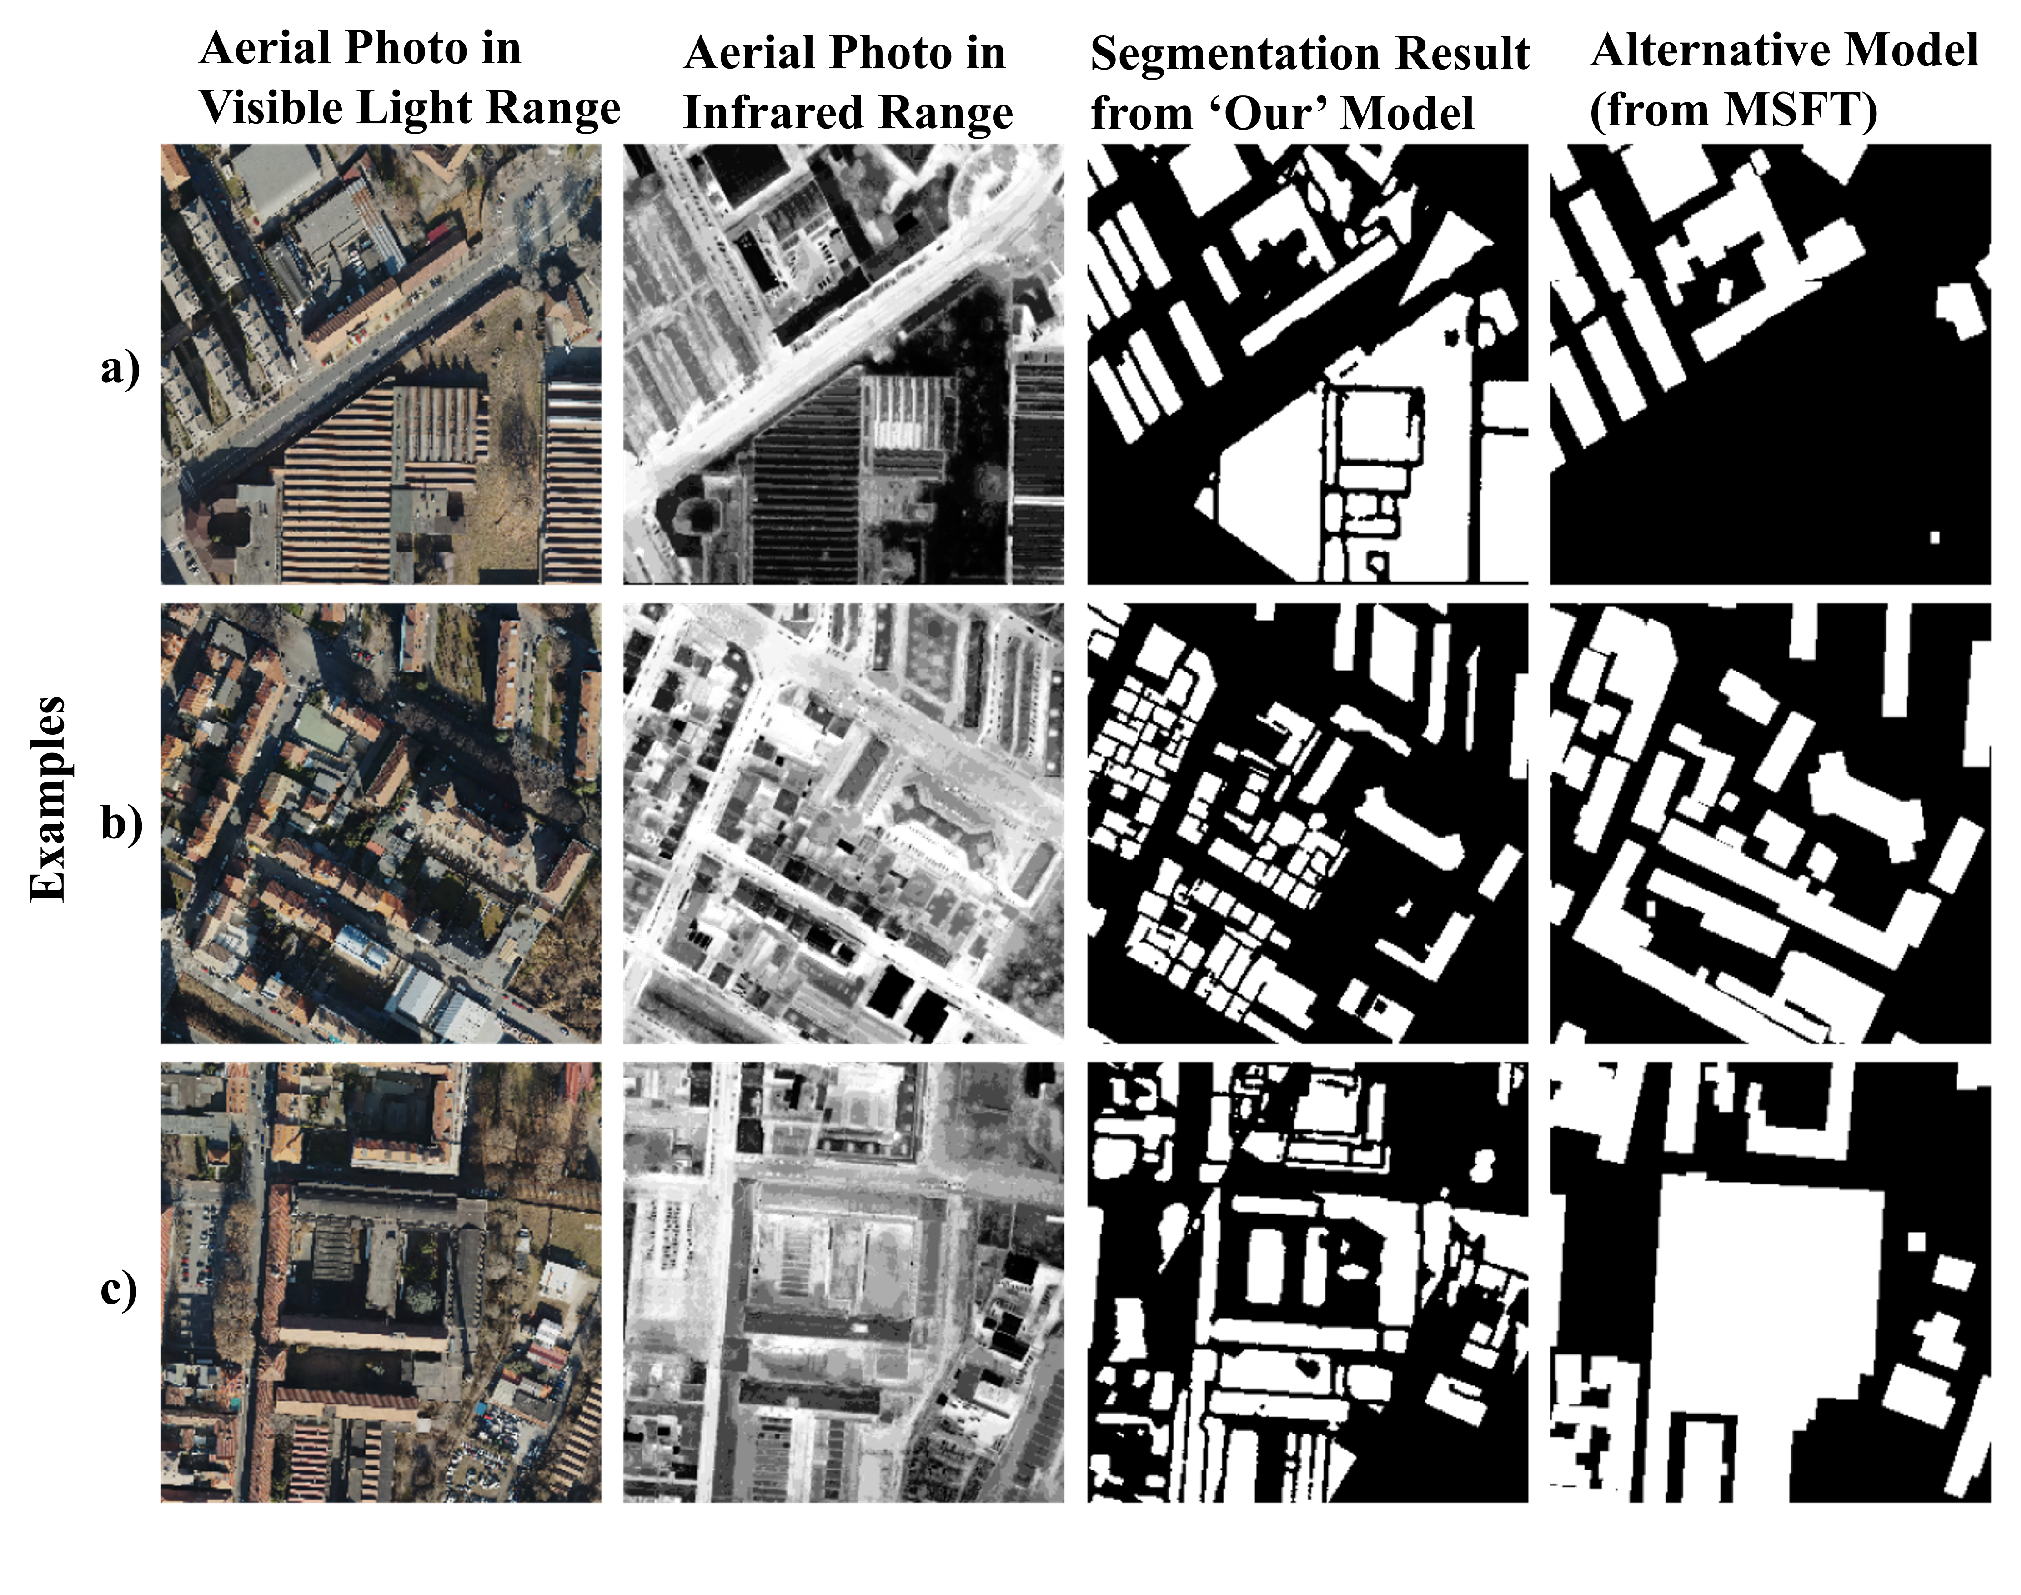
\includegraphics[height=0.75\linewidth]{img/compre_results.pdf}
    \caption{Results from Segmentation shown with thermal image heat map alongside Microsoft (MS) Footprints}
    \label{fig:segresults}
    \end{figure}
    
    \subsection{Modeling Results}%CLC
    Table~\ref{tab:model_comparison_top7} shows the resulting metrics from our top-performing models in terms of RMSE and MAE are the Random Forest Regressor, Extra Trees Regressor, and CatBoost Regressor. These ensemble models likely outperform the others due to their ability to capture complex non-linear relationships between the features and the target variable, as well as their robustness to outliers and noise in the data. As our ultimate goal in setting up this regression problem, we do aim at classifying buildings into different EUI bins. At such the CatBoost Regressor might be the most desirable choice, as it combines the strengths of both decision trees and gradient boosting, and has been shown to perform well in various classification tasks. 

    \begin{table}[h!]
    \centering
    \resizebox{\textwidth}{!}{%
    \begin{tabular}{|l|l|c|c|c|c|c|}
    \hline
    \textbf{Model} & \textbf{Model} & \textbf{MAE }& \textbf{MSE} & \textbf{RMSE} & \textbf{RMSLE} & \textbf{MAPE} \\ \hline
    rf & Random Forest Regressor & 27.20 & 1166.58 & 33.99 & 0.22 & 0.19 \\ \hline
    omp & Orthogonal Matching Pursuit & 27.35 & 1173.23 & 34.08 & 0.23 & 0.19 \\ \hline
    dummy & Dummy Regressor & 27.43 & 1174.30 & 34.09 & 0.23 & 0.19 \\ \hline
    et & Extra Trees Regressor & 27.20 & 1175.31 & 34.11 & 0.23 & 0.19 \\ \hline
    catboost & CatBoost Regressor & 27.10 & 1194.77 & 34.38 & 0.23 & 0.19 \\ \hline
    ada & AdaBoost Regressor & 27.70 & 1202.22 & 34.49 & 0.23 & 0.20 \\ \hline
    gbr & Gradient Boosting Regressor & 27.63 & 1210.77 & 34.65 & 0.23 & 0.19 \\ \hline
    \end{tabular}%
    }
    \caption{Alternative model comparison (top 7) from AutoML Pipeline}
    \label{tab:model_comparison_top7}
    \end{table}

    \paragraph{Predictive accuracy and practical relevance.} Table~\ref{tab:model_comparison_top7} shows that the CatBoost model predicts \emph{per–building} energy-use intensity with an RMSE of 34.4~kWh\,m$^{-2}$\,yr$^{-1}$ (MAPE 19\,\%). A bin-by-bin comparison against the official EPC energy classes~(A--G) reveals an overall classification accuracy of 62\,\%. Misclassifications are overwhelmingly \emph{adjacent}: 93\,\% of errors fall within $\pm1$~energy band, implying the model seldom confuses, say, a ``B'' building for an ``E'' one. The mean signed error is $-4.1$~kWh\,m$^{-2}$\,yr$^{-1}$, indicating a slight conservative bias that errs on the side of over-estimating consumption---a desirable property for retrofit prioritisation.  Errors increase with very low EUIs ($<40$ kWh\,m$^{-2}$\,yr$^{-1}$), where façade heat loss approaches the noise floor of the sensor (cf.\ standard deviation column in Table~\ref{tab:eui-metrics}); in all other bands the interquartile error remains within $\pm$21~kWh\,m$^{-2}$. These results place the proposed thermal-only approach mid-range among recent EPC-only benchmarks (24--40~kWh\,m$^{-2}$\,yr$^{-1}$ RMSE) while requiring \emph{no} on-site data.

    It is important to note the current case study aims at demonstrating the feasibility of using thermal imagery and machine learning techniques for EUI prediction. As we have not used any other features that are available from the EPCs, it is plausible to speculate that combining additional EPC-originating features can allow for the current pipeline to perform better. However, as the challenge of cleaning up and collapsing multiple rows of EPC records into one is beyond of the scope of the current study and defeates our purpose, we opted to not investigate the matter any further and only reported the results that leverages EPCs as source of our labels. Moreover, we have also tested other approaches to engineer features such as clustering the thermal images as well as leveraging various deep learning techniques, but the improvements observed is minimal on top of results shown in Table~\ref{tab:model_comparison_top7}.%Future studies could explore the potential synergies between these two data sources and develop more sophisticated models that leverage the strengths of both thermal imagery and EPC data for accurate and reliable EUI prediction.

\section{Limitations and Future Outlooks}
    % \subsection{Segmentation Algo Improvements?}
    It is important to contextualize the specific operational limitations detailed below with some fundamental constraints of this study, as highlighted in Section 2.4. Firstly, the predictive model, while promising, is inherently tailored to the building typologies, urban landscape, and climate zone characteristic of Turin; its direct transferability to areas with different profiles may therefore be limited without further validation or recalibration. Secondly, thermal imagery analysis is subject to the influence of surface emissivity, which can vary significantly with material properties and environmental conditions (such as surface moisture) and thus affect the accuracy of temperature measurements. These broader considerations, alongside the subsequent points, inform the scope of our findings and the directions for future work.
. These factors, alongside the specific issues detailed below, frame the context for future research directions.
    \subsection{Points and Polygon Alignment}%CLC
    Initially, our attempt in aligning the point features (X, Y coordinates from EPC data) with polygons (segmentation-identified footprints) was unsuccessful. Although it was anticipated that most of the points are not going to be sitting perfectly within the segmented footprints, we were still surprised by identifying approximately 17\% of points (~200 out of ~1200) will sit inside the polygons, ergo a majority of points landed outside of our segmented patches. Even as we expanded the points to polygons that are closest to it, the result of number of polygons used was still limited, with only about 25\% of polygons (~300) out of all polygons we identified. This resulted in a significant reduction in usable surface temperature information from our raster sheet. Upon reviewing the results, we believe this suggest our initial plan of conducting point-to-polygon alignment for EUI prediction needed to be revised. The reduced efficacy of using segmented-thermal-patch-based information for predicting EUIs points to the need to explore alternative approaches that can effectively capture the nuances from the thermal imagery. 

    At such, we decided to switch to a polygon-to-point strategy. This strategy offers a promising solution by leveraging all possible surface temperature information in our dataset. In our new approach, each polygon is associated with its closest point(s), utilizing only data related to their respective locations and EUI values. This method effectively circumvents the limitations of spatial join due to latitude/longitude errors, enabling the creation of a more robust and informative dataset for machine learning model training. However, this approach may introduce biases if the polygons are not accurately representative of the underlying building characteristics or thermal behavior in our study, or being linked to points that are in fact from an adjacent building whose thermal characteristics are drastically different. The reliance on location and EUI data alone might overlook important contextual information that is essential for accurate predictions. Nonetheless, associating each polygon with its closest point(s), we were able to create datasets that are more suitable for model training, enabling prediction of EUI values based on segmented-thermal-patch-based information alone. With the omission of any other information aside from the EUIs calculated, we are foregoing many different dimensions from the EPCs that might be helpful, including year of construction, type of system/façade, etc. that might be very helpful in improving the EUIs for our study.

    This shift from one alignment strategy to another helped us by eliminating the need to reconcile discrepancies in contextual information from EPC records. In other words, should more columns to be leveraged, a consistent strategy that helps us 'collapse' different field values within the same column from multiple EPC records into one needs to be devised. This is particularly challenging as it's extremely difficult to identify an appropriate 'dropping' strategy on deciding what values to keep and what to be deserted when lacking the right values as 'ground truth'. By abandoning the point-to-polygon strategy, we were able to on developing and refining our model without these added complexity. Future research should nonetheless attempt again at improving point-to-polygon alignment methods and data reconciliation approach to better predict building-level thermal behavior. More robust alignment techniques could provide more accurate predictions of EUI values. These contextual factors are crucial for capturing the nuances of building-level energy behavior. 

\section{Conclusion}
    This framework demonstrates how municipalities can leverage automated thermal assessment to transform retrofit planning from reactive, building-by-building approaches to proactive, district-scale strategies. By delivering actionable energy performance insights from a single aircraft campaign, our approach enables rapid screening of entire neighborhoods—addressing the EU Green Deal's ambitious timeline for building renovation at unprecedented scale and cost-effectiveness. The Turin demonstration validates the potential for EU-wide deployment, offering municipal planners a scalable alternative to traditional energy audits that require neither site visits nor specialized building expertise. Our experimental results benchmark thermal imagery-based predictions against traditional EPC-based approaches, using EPC data solely to calculate target EUIs and geolocate buildings. In addressing our opening questions, we have shown the following:
    
    \begin{enumerate}
        \item Thermal imagery segmentation using unsupervised multi-modal models does provide valuable information for remote-sensing based  assessments. The segmentation process allows for a more detailed understanding of building-level energy performance, revealing patterns and anomalies that may be overlooked in traditional EPC data.
        \item The segmented thermal imageries alone can be used  to create a model that can predict EUI with a comparative accuracy to some state-of-the-art models that are EPC-based. It is highly likely that with the two further integrated, we can create a more comprehensive pipeline instead of only extracting EUI labels for predicting energy consumptions as seen the current study.
        \item The implications of our approach are significant for both urban energy policy and planning. Policymakers can be empowered by a highly-scalable solution like ours to prioritize energy efficiency while allocate resources, allowing for our approach to further encourage energy-efficiency building practices, starting with detecting buildings that are in need for energy audits.
    \end{enumerate}
    
    While our results demonstrate the effectiveness of using thermal imagery captured in March, we acknowledge a limitation in capturing seasonal variations, such as peak winter heating demands or summer cooling loads. Future studies should consider extending data acquisition to multiple seasons or developing seasonal adjustment factors to enhance prediction accuracy across varying climatic conditions. This would significantly improve the robustness and applicability of our methodology in diverse urban environments.
    
    Furthermore, our study heavily focused on data quality and alignment in the integration process. In discussing the alignment issue between EPC-based points and segmentation-resulting polygons, we paved an important opening to additinoal future studies in addressing similar challenges. In addition, our study highlights several critical avenues for further investigation. Although our thermal imagery-based model demonstrates promising accuracy, its current evaluation is constrained by the use of a single thermal snapshot and the inherent noise from aggregating EPC data. Future work will integrate multi-temporal thermal datasets to capture seasonal variations, thereby providing a more robust validation of our approach. Furthermore, our unsupervised segmentation pipeline and AutoML-based modeling framework offer a scalable and replicable solution that can be extended to broader urban contexts. We plan to benchmark our methodology against established physics-based and traditional regression models to further substantiate its efficacy. Overall, these developments will pave the way for a comprehensive, data-driven strategy for urban energy assessment, with significant implications for energy policy and sustainable urban planning.
    
    In conclusion, we demonstrated how thermal imagery can enable municipal energy planning through remote-sensing based EUI prediction. The highly scalable unsupervised segmentation pipeline developed here has potential to revolutionize urban energy assessment across diverse European contexts. As cities worldwide face pressure to meet climate targets, our research provides municipal decision-makers with evidence-based tools for retrofit prioritization and sustainable urban energy system development. Future multi-city validation across different European building stocks will further establish this approach as a cornerstone technology for the EU's building renovation wave.

\section{Acknowledgement}    
    This paper reports part of the work developed within the project NODES, which has received funding from the MUR - M4C2 1.5 of PNRR with grant agreement no. ECS00000036. The authors would also like to thank the support from the Department of Architecture, Faculty of Architecture for the research support that enabled this research.
% \listoftodos

 \bibliographystyle{elsarticle-num} 
 \bibliography{EPC_Segmentation}

%% else use the following coding to input the bibitems directly in the
%% TeX file.

% \begin{thebibliography}{00}

% %% \bibitem{label}
% %% Text of bibliographic item

% \bibitem{}

    
% \end{thebibliography}
\end{document}
\endinput
%%
%% End of file `elsarticle-template-num.tex'.
